\documentclass[dissertation.tex]{subfiles}
\begin{document}

\section{Success Criteria}

The project was a success. I have met all the success criteria specified in the
proposal. That is, I have reproduced the experiments presented in Tishby's paper.
I have produced a software suite that can run configurable experiments and can
be extended in the future.

\section{Extensions}

I have achieved a number of extensions for the project:

\begin{itemize}
  \item{
      Investigated the ideas presented in paper by Saxe. Devised an experiment
      that contradicts Saxe's conclusion about compression. See
      \autoref{subEvalSaxe}
    }
  \item{
      Devised and Implemented Batching MIE. A method that aims to increase
      accuracy of currently available mutual information estimation techniques .
      See \autoref{subEvalBatching}.
    }
  \item{
      Extended the code to accommodate for different MIE. Added KDE MIE as an
      KDE was used by Saxe in his paper, my implementation follows the code
      verbatim. Adding more different MIEs requires writing code, but is doable.
    }
  \item{
      Extended the code to accommodate for different datasets and added the
      MNIST dataset as an option. Adding more datasets requires writing code,
      but is easily done.
    }
  \item{
      Extended the code to be able to use different MIE on the same instance of
      a NN, in order to be able to compare how they perform. Previously to
      compare MIEs we either needed to save information for the whole training
      period of a NN or to launch two different instances of a NN with the same
      parameters, which might yield different results.
    }
  \item{
      Extended the code to improve performance.
      \begin{itemize}
        \item{
            Made the code parallel -- information for multiple epochs can be
            computed at the same time.
          }
        \item{
            Introduced adaptive ways to skip MI computations, which speed up
            computation significantly.
          }
      \end{itemize}
    }
  \item{
      Implemented movie plotting tools, which allow us to see how information
      plane changes over the training period. This allows us to better analyse
      the data and detect any issues we may have.
    }
\end{itemize}


\section{Tishby's Experiment}

In the implementation chapter we discussed the importance of randomness and
noise for compression within Neural Networks. We introduced Mutual Information
Estimator and set up our tool chain. This allows us to investigate and try to
reproduce the specific experiment conducted by Tishby and Saxe.

In order to reproduce Tishby's work I have to compute the MI information values
$I(X, T_{e,l})$ and $I(Y, T_{e,l})$ for the specific hyperparameters he used.
This will allow me to plot the Information Plane and analyse the results.  In
order to show the results are robust I tune the hyperparameters and see if the
results change significantly. Tishby used the following default hyperparameters:
MIE - Binning, Dataset\footnote{I did not have the time to test if the results
are robust to changes in the dataset.  However, the tools provide a way to
natively run the MNIST dataset and adding more is reasonably simple.} -
Tishby's, Training Size - 40\%, activation function - $\tanh$, batch size - 512,
network shape 12,10,8,6,4,2 (how many node in every layer). Throughout this
section if any of the hyperparameters are not specified assume they are the
default values. 

I claim to have successfully reproduced the results if the generated Information
Plane looks similar \autoref{figIplane} and the it follows the loose definitions
of \emph{Compression Phase} and of \emph{Fitting Phase} as described in
\autoref{subIotIP}. I have successfully reproduced Tishby's results for his
default hyperparameters and have showed the results are robust for:
\begin{itemize}
  \item{
      Training size, \autoref{figTS}. Note that higher training set implies we
      can learn more about the label, this is exactly what we see.
    }
  \item{
      Network Shape, \autoref{figNetworkShapes}. Note that amount of compression
      seems to be highly correlated with the size of the data layer size to the
      point where we cannot distinguish most of the early layers apart.
    }
  \item{
      Batch Size, \autoref{figBatchSize}. The results seem to be very robust to
      batch size as the graphs all look very similar. 
    }
  \item{
      Bin count for the Binning MIE, \autoref{figBinCount}. If we increase the
      number of bins we reduce the noise in the network and hence get less
      compression visible. We see exactly this in the figures for Bin count >
      30. It seems that for high value of Bin count we we capture all the
      information about the input and the label. Nevertheless, the compression
      phase still appears to happen.
    }
\end{itemize}

However, changing MIE and the activation function and produced results that were
not inline with the ideas Tishby presented.

% Binning Training Set
\begin{figure}[ht]
  \centering
  \begin{subfigure}[t]{0.32\textwidth}
    \centering
    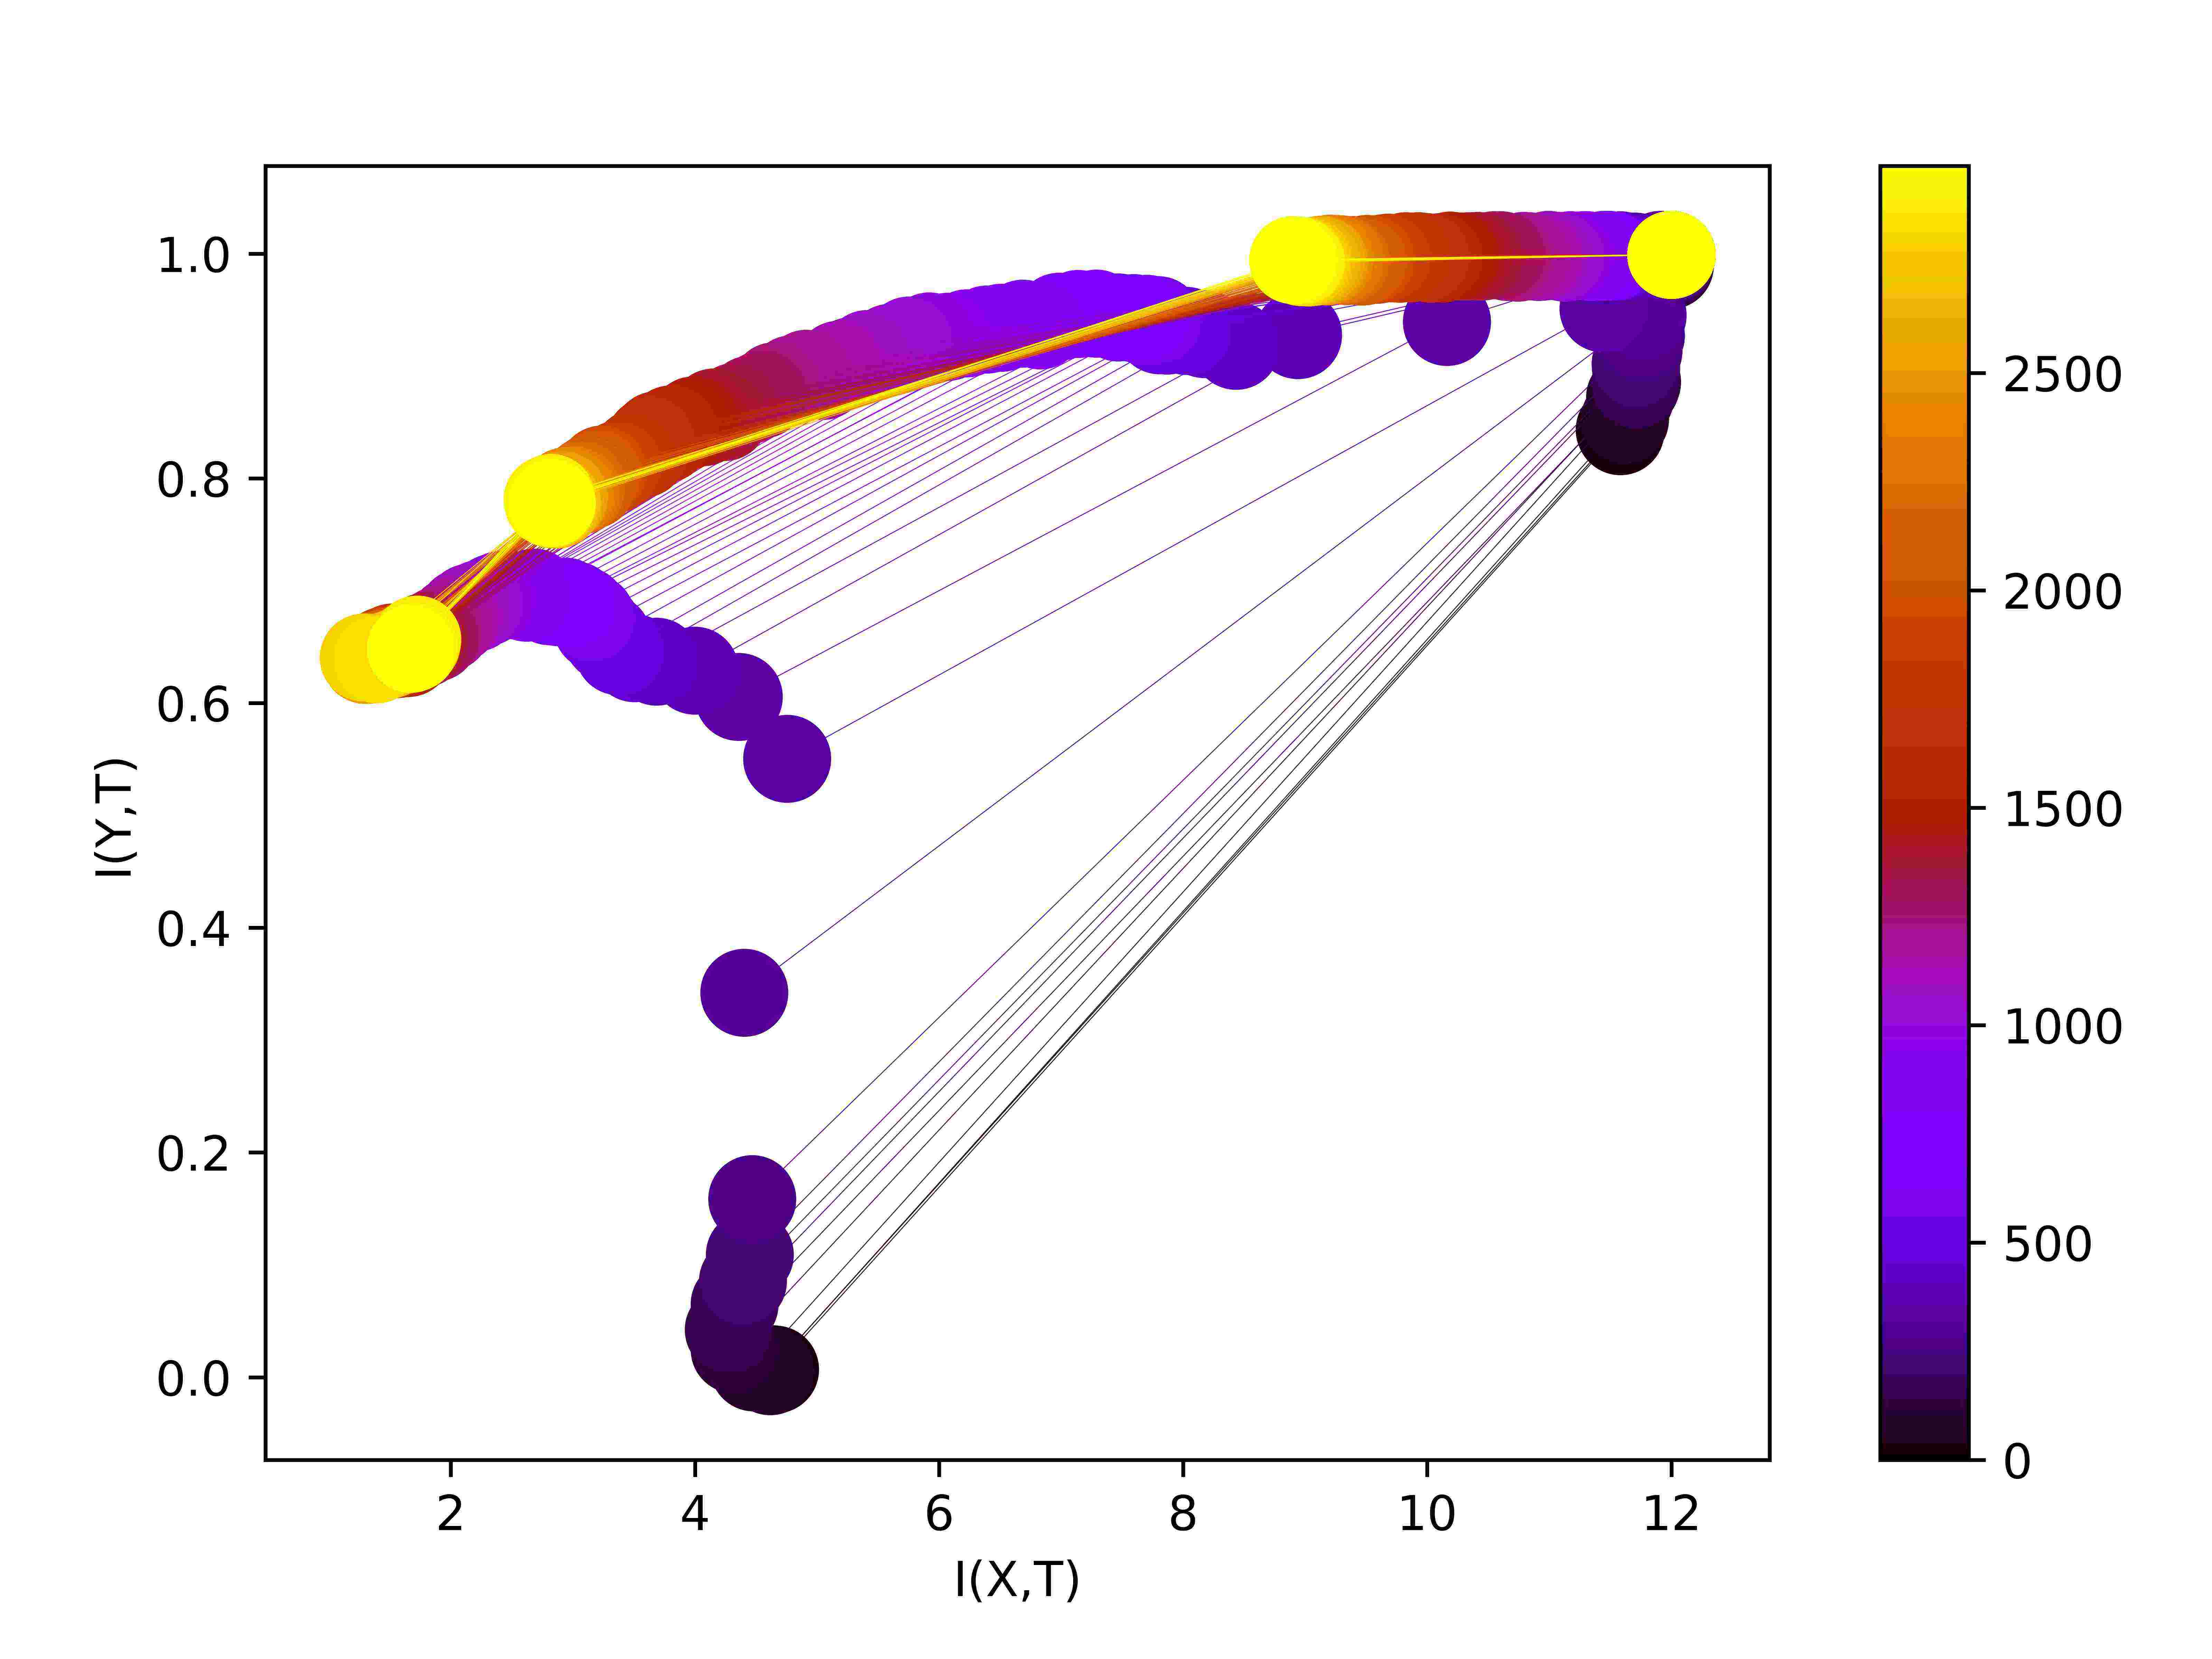
\includegraphics[width=\textwidth]{figs/eval/trainingSize/Binning20.jpg}
    \caption{
      Training size - 20\%
    }
    \label{figBinningTS20}
  \end{subfigure}
  \begin{subfigure}[t]{0.32\textwidth}
    \centering
    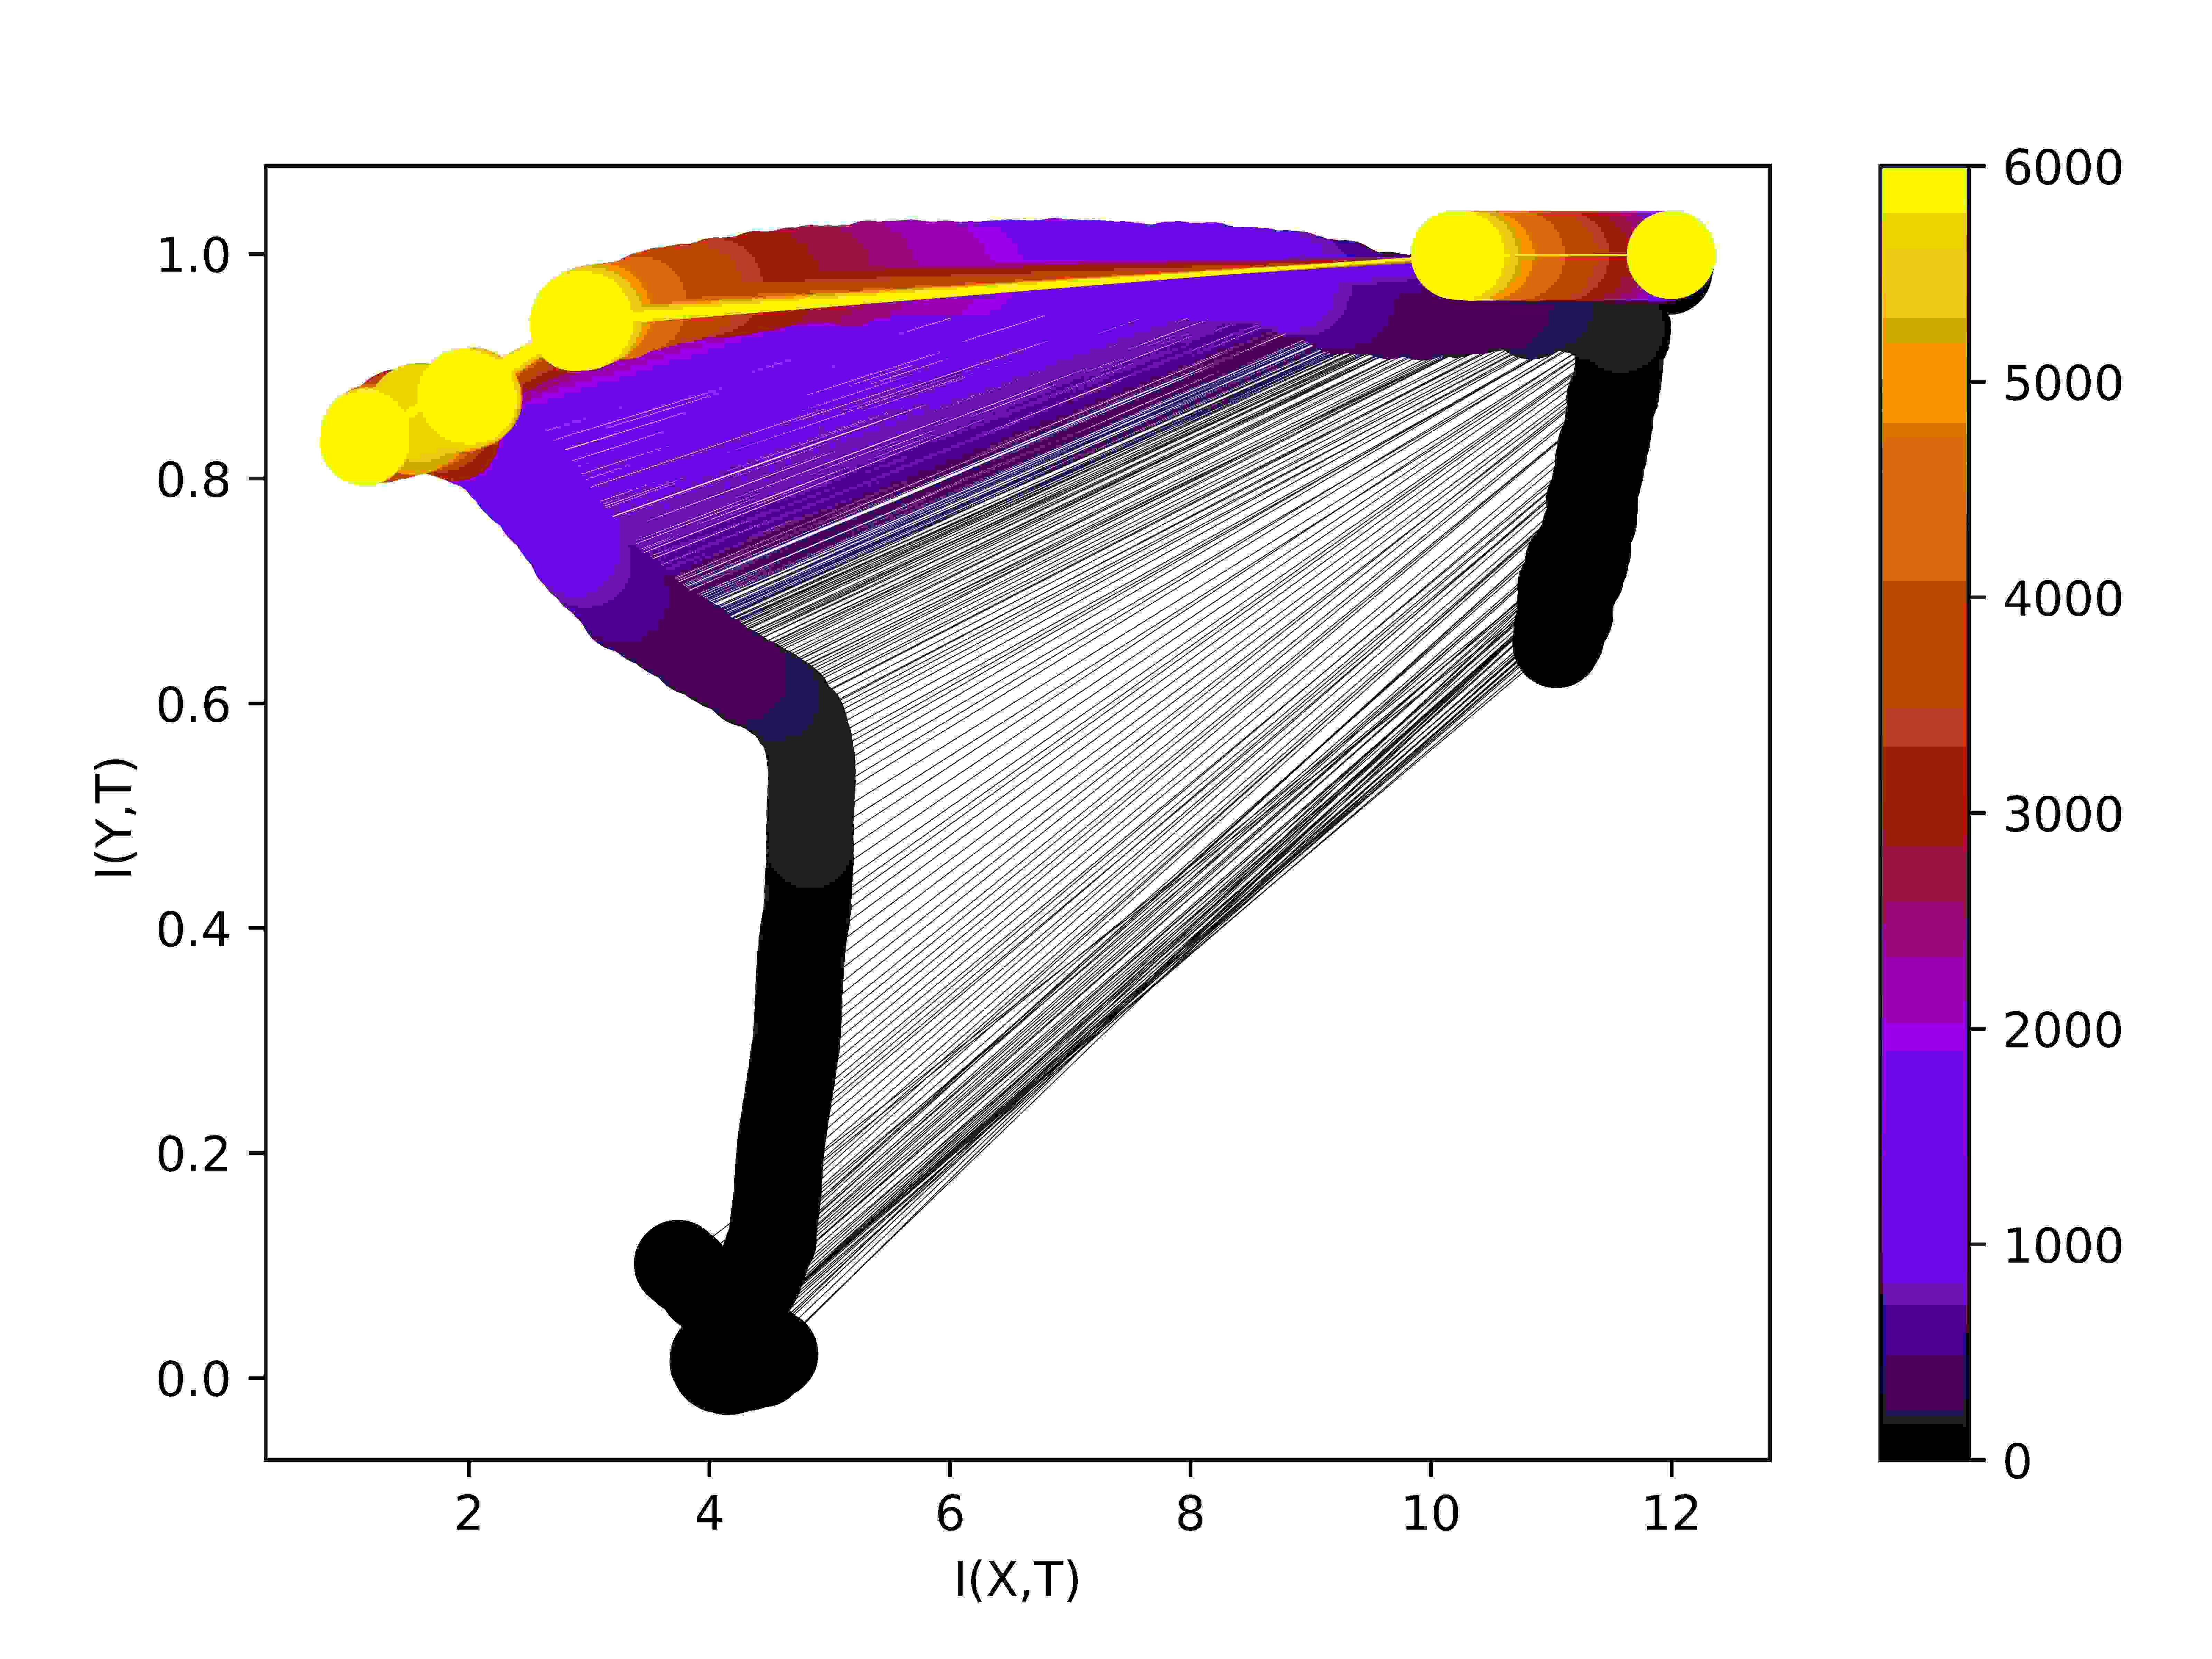
\includegraphics[width=\textwidth]{figs/eval/trainingSize/Binning40.jpg}
    \caption{
      Training size - 40\%
    }
    \label{figBinningTS40}
  \end{subfigure}
  \begin{subfigure}[t]{0.32\textwidth}
    \centering
    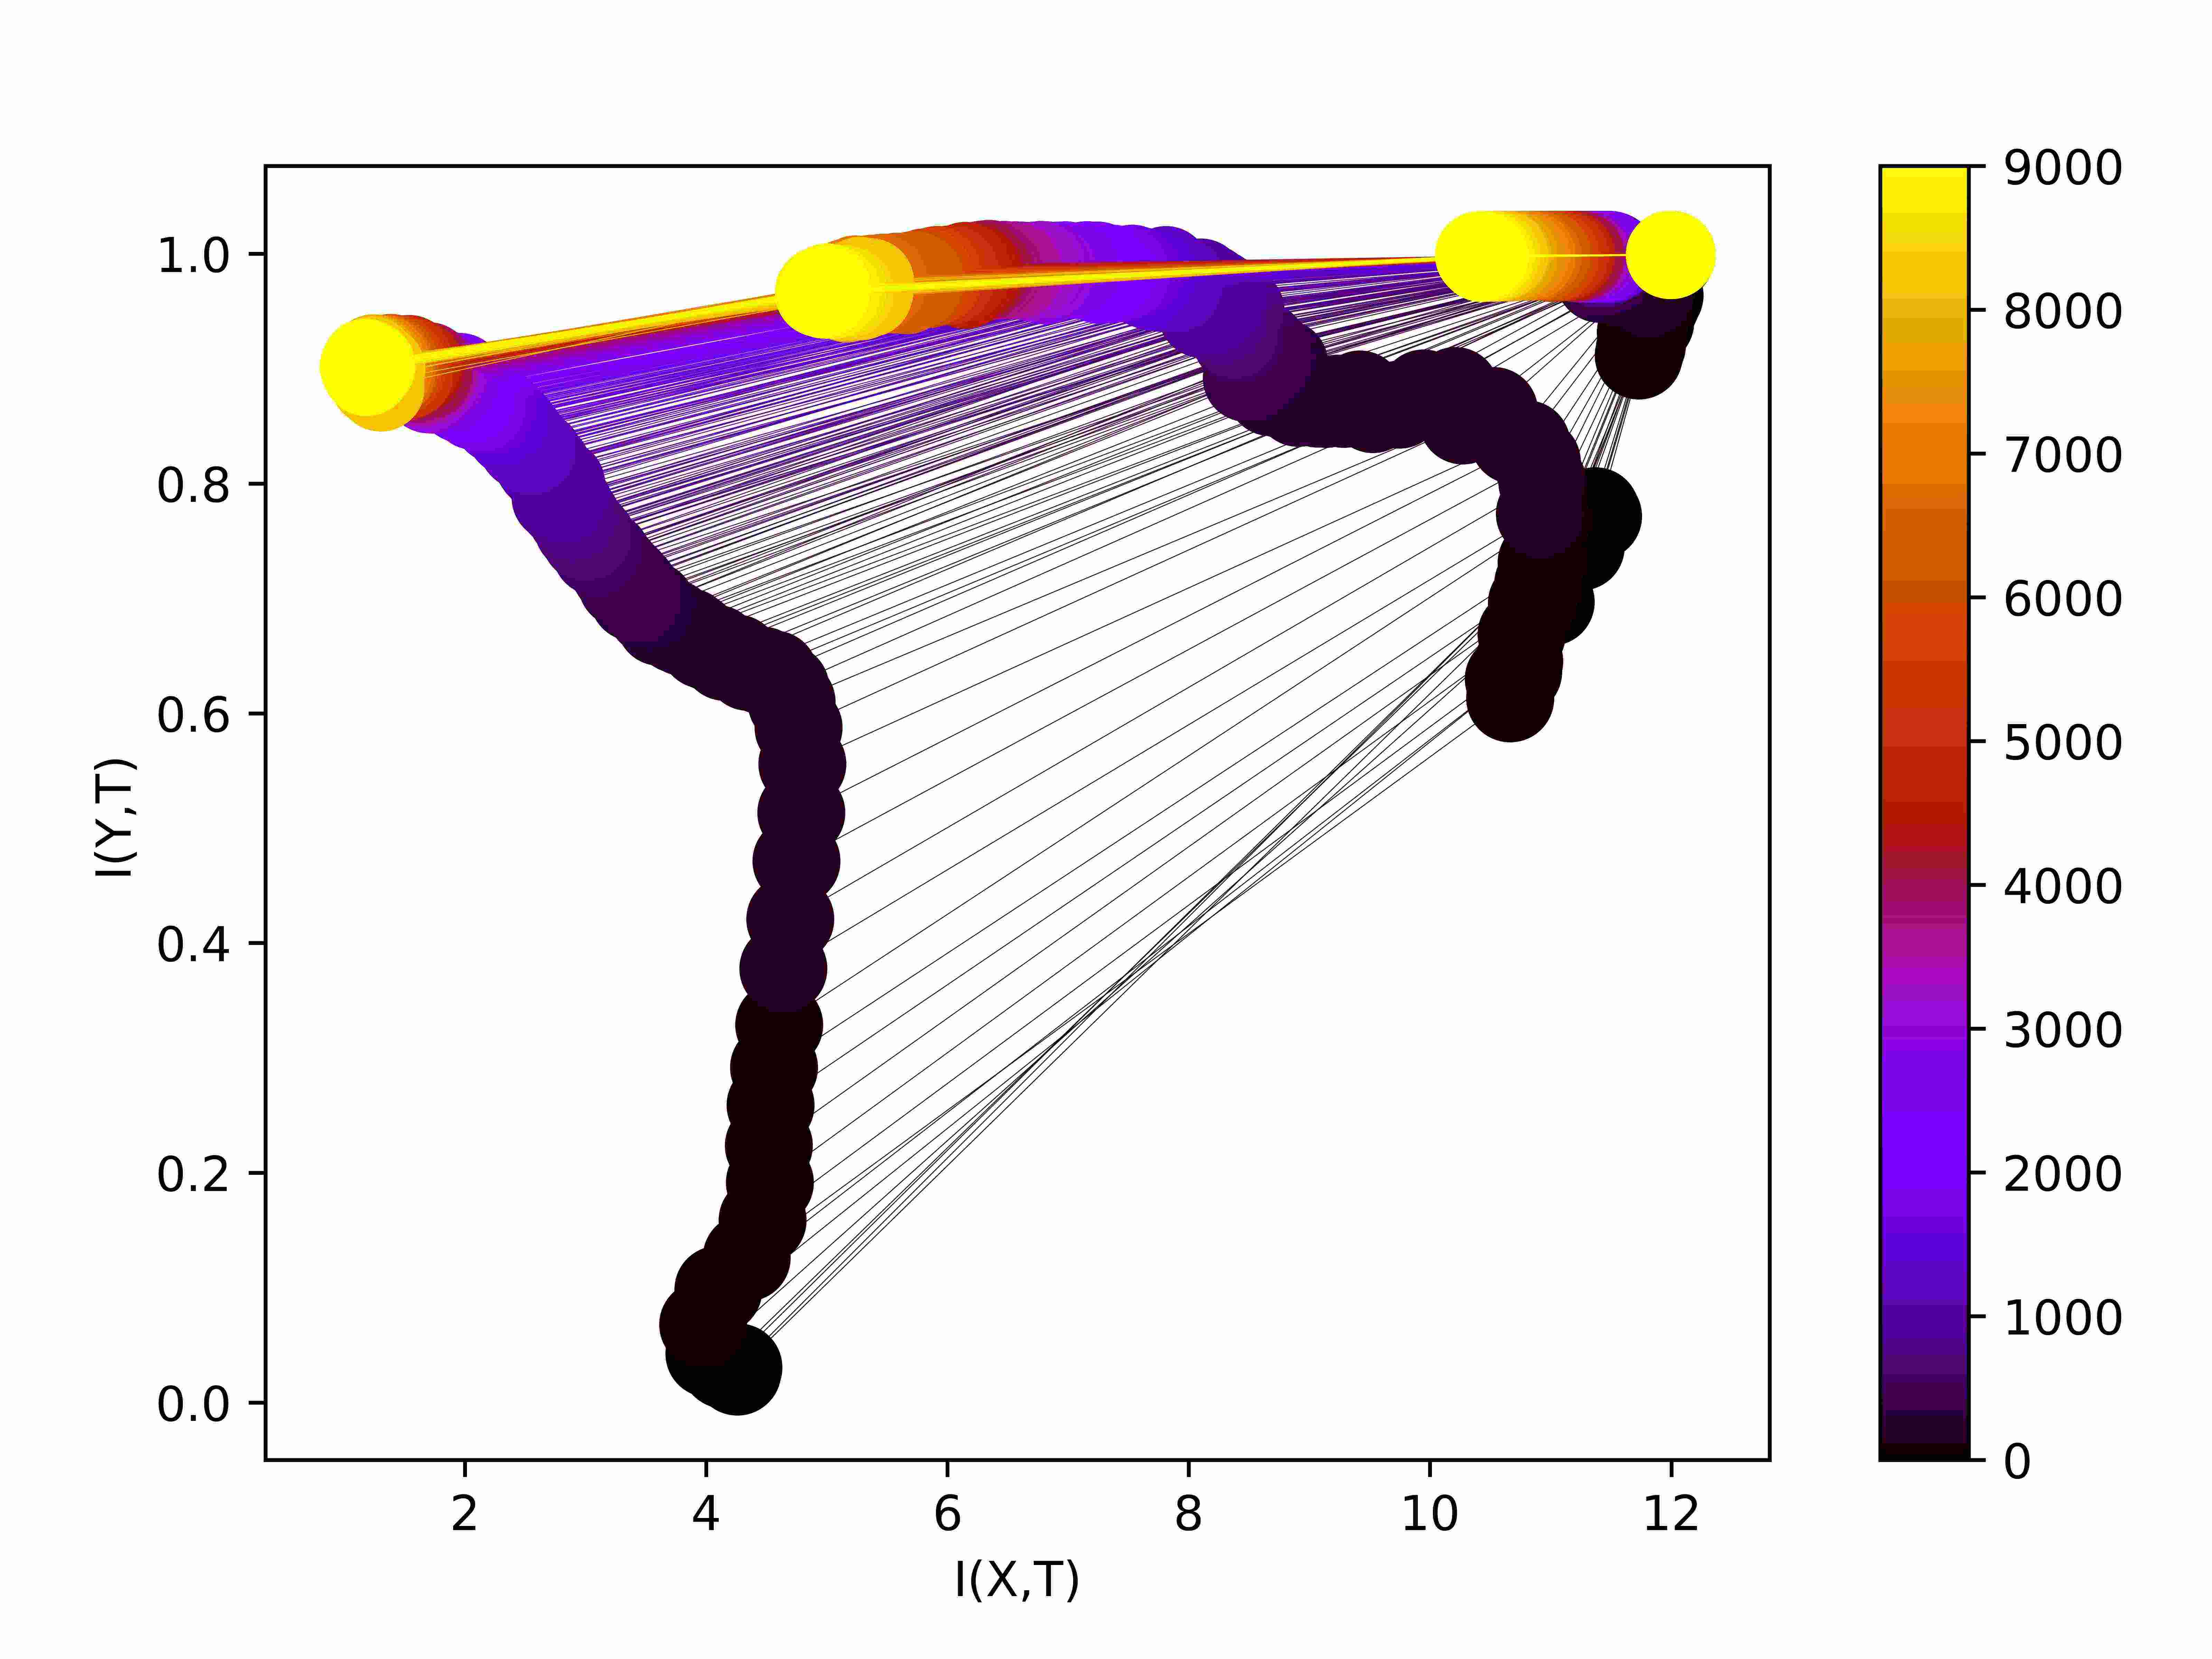
\includegraphics[width=\textwidth]{figs/eval/trainingSize/Binning70.jpg}
    \caption{
      Training size - 70\%
    }
    \label{figBinningTS70}
  \end{subfigure}
  \caption{
      Tweaking training size for Tishby's binning MIE.
    }
  \label{figTS}
\end{figure}

\begin{figure}[ht]
  \centering
  \begin{subfigure}[t]{0.32\textwidth}
    \centering
    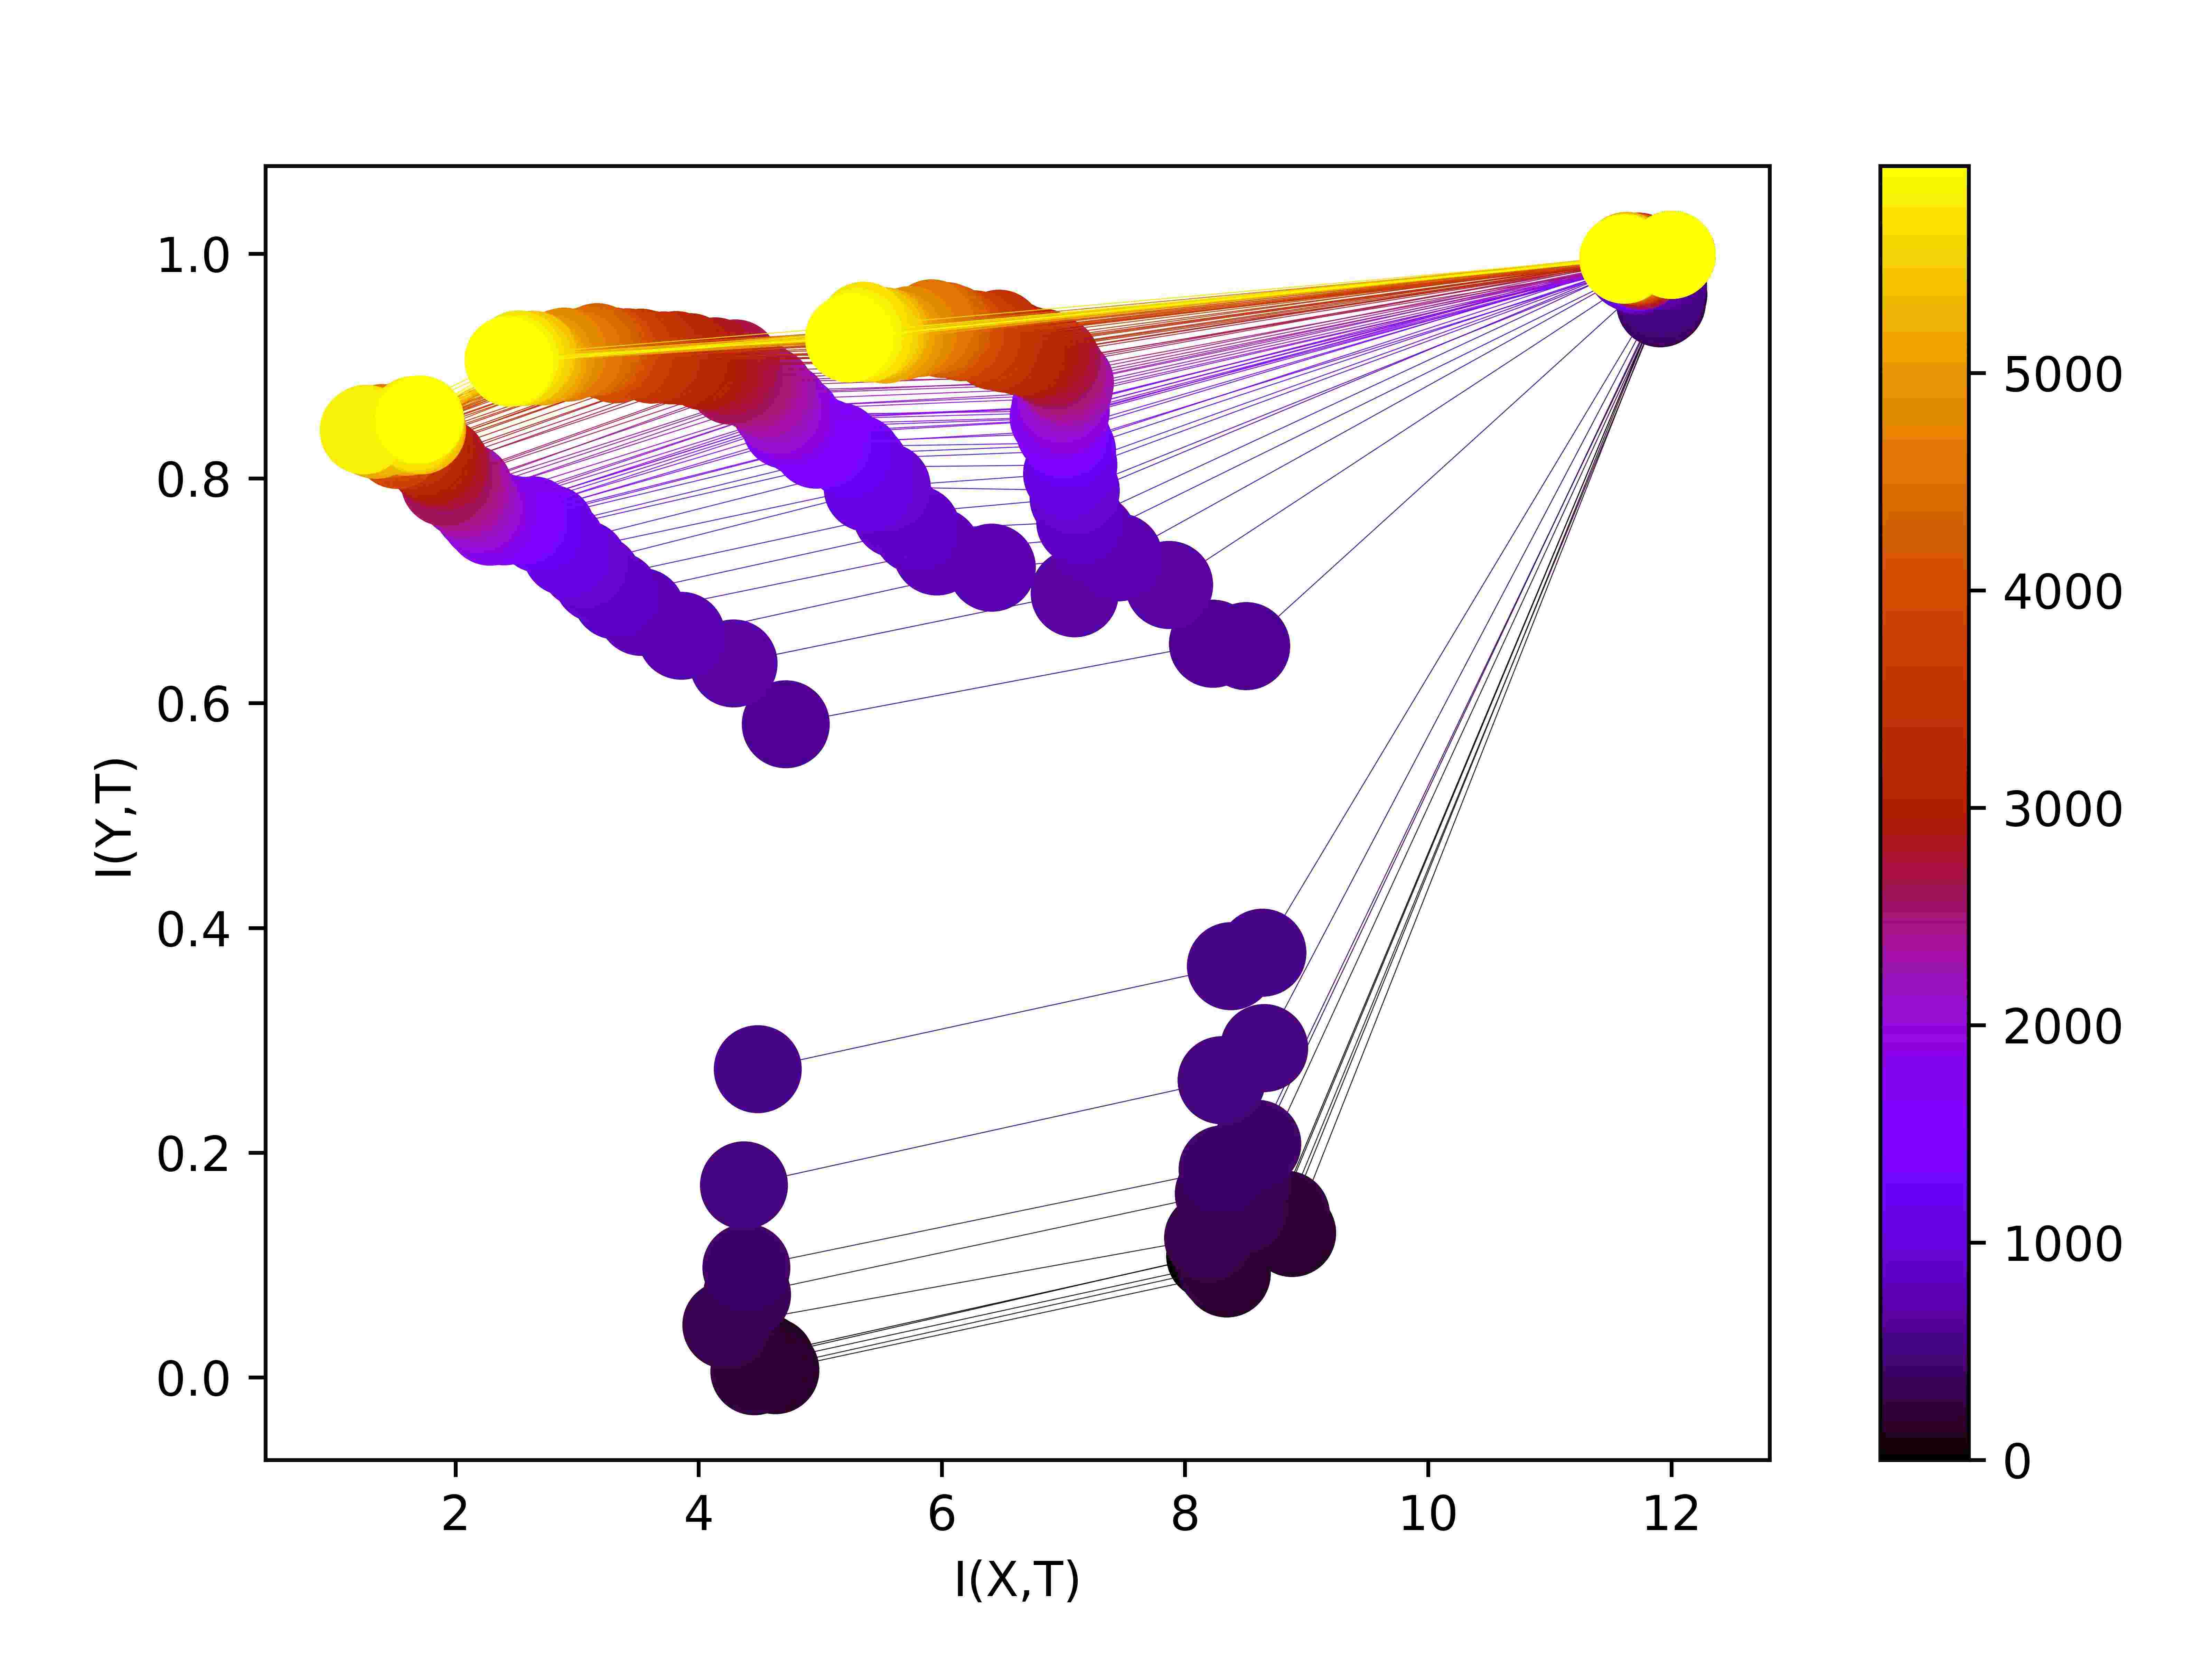
\includegraphics[width=\textwidth]{figs/eval/networkShape/Binning10,4,2,2.jpg}
    \caption{
      Network Shape - 12,10,4,2,2,2
    }
    \label{figNetworkShapeDefault}
  \end{subfigure}
  \hfill
  \begin{subfigure}[t]{0.32\textwidth}
    \centering
    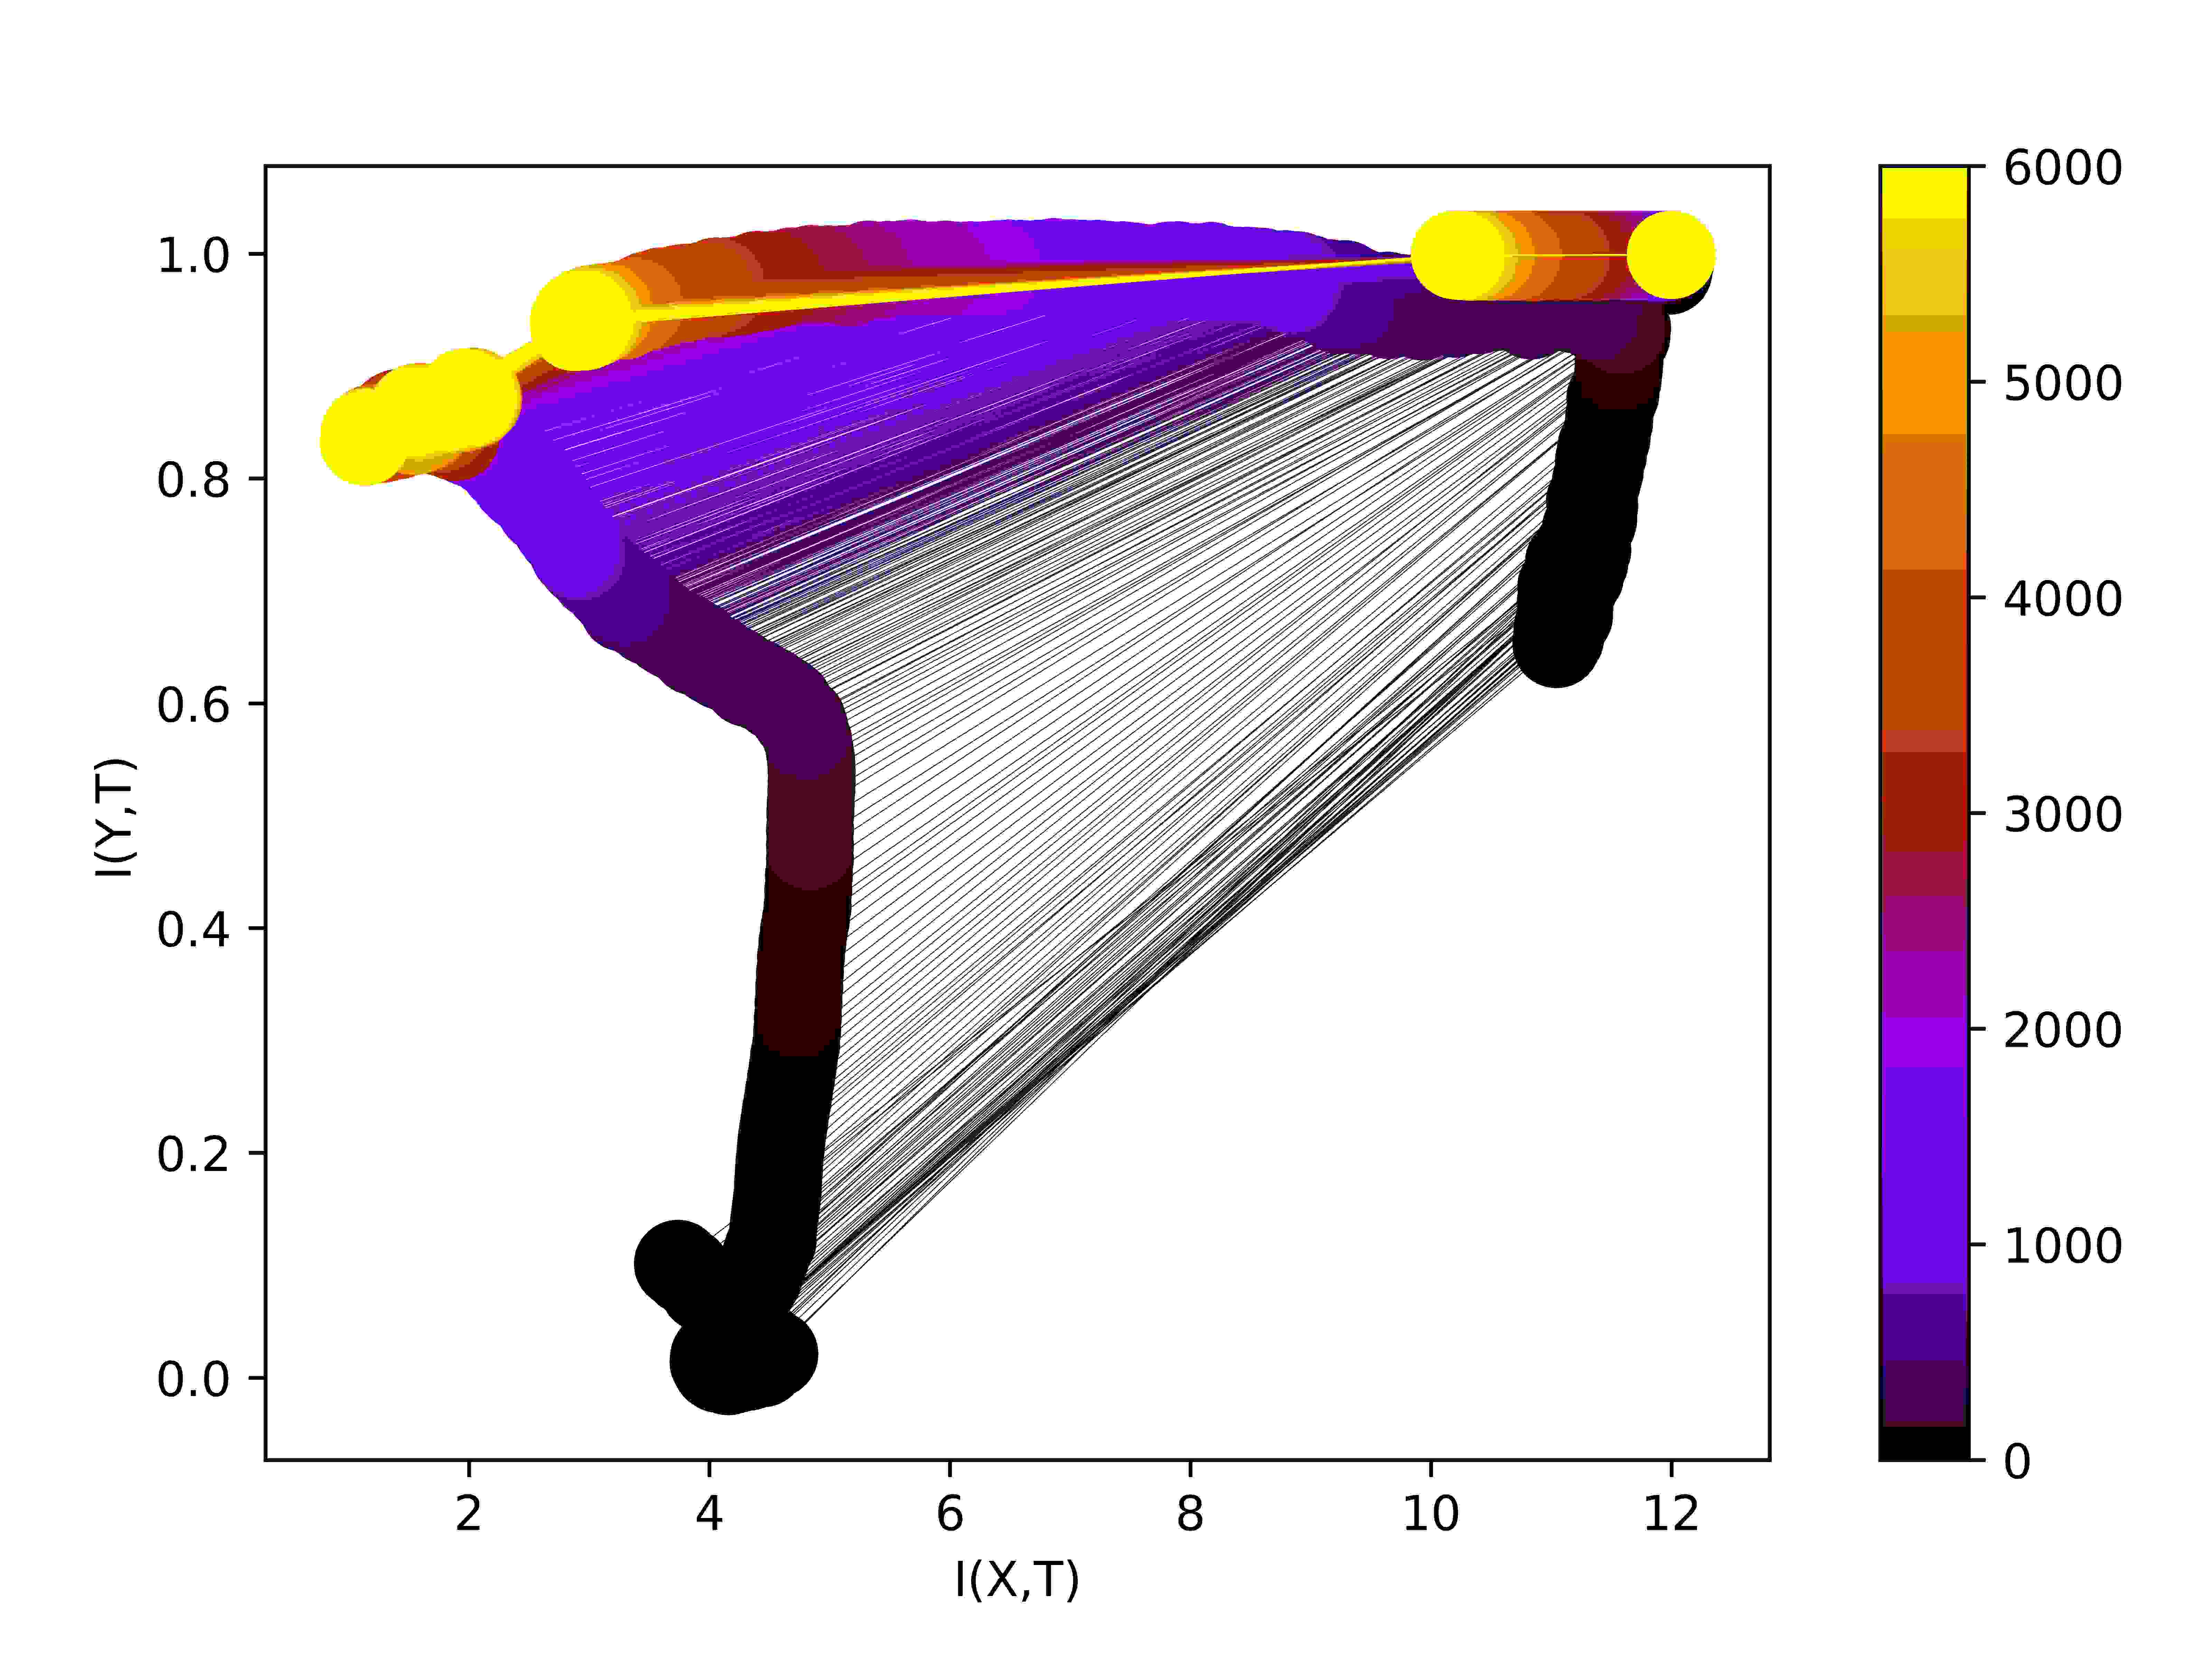
\includegraphics[width=\textwidth]{figs/eval/networkShape/Binning10,8,6,4.jpg}
    \caption{
      Network Shape - 12,10,8,6,4,2, Default
    }
    \label{figNetworkShape2}
  \end{subfigure}
  \hfill
  \begin{subfigure}[t]{0.32\textwidth}
    \centering
    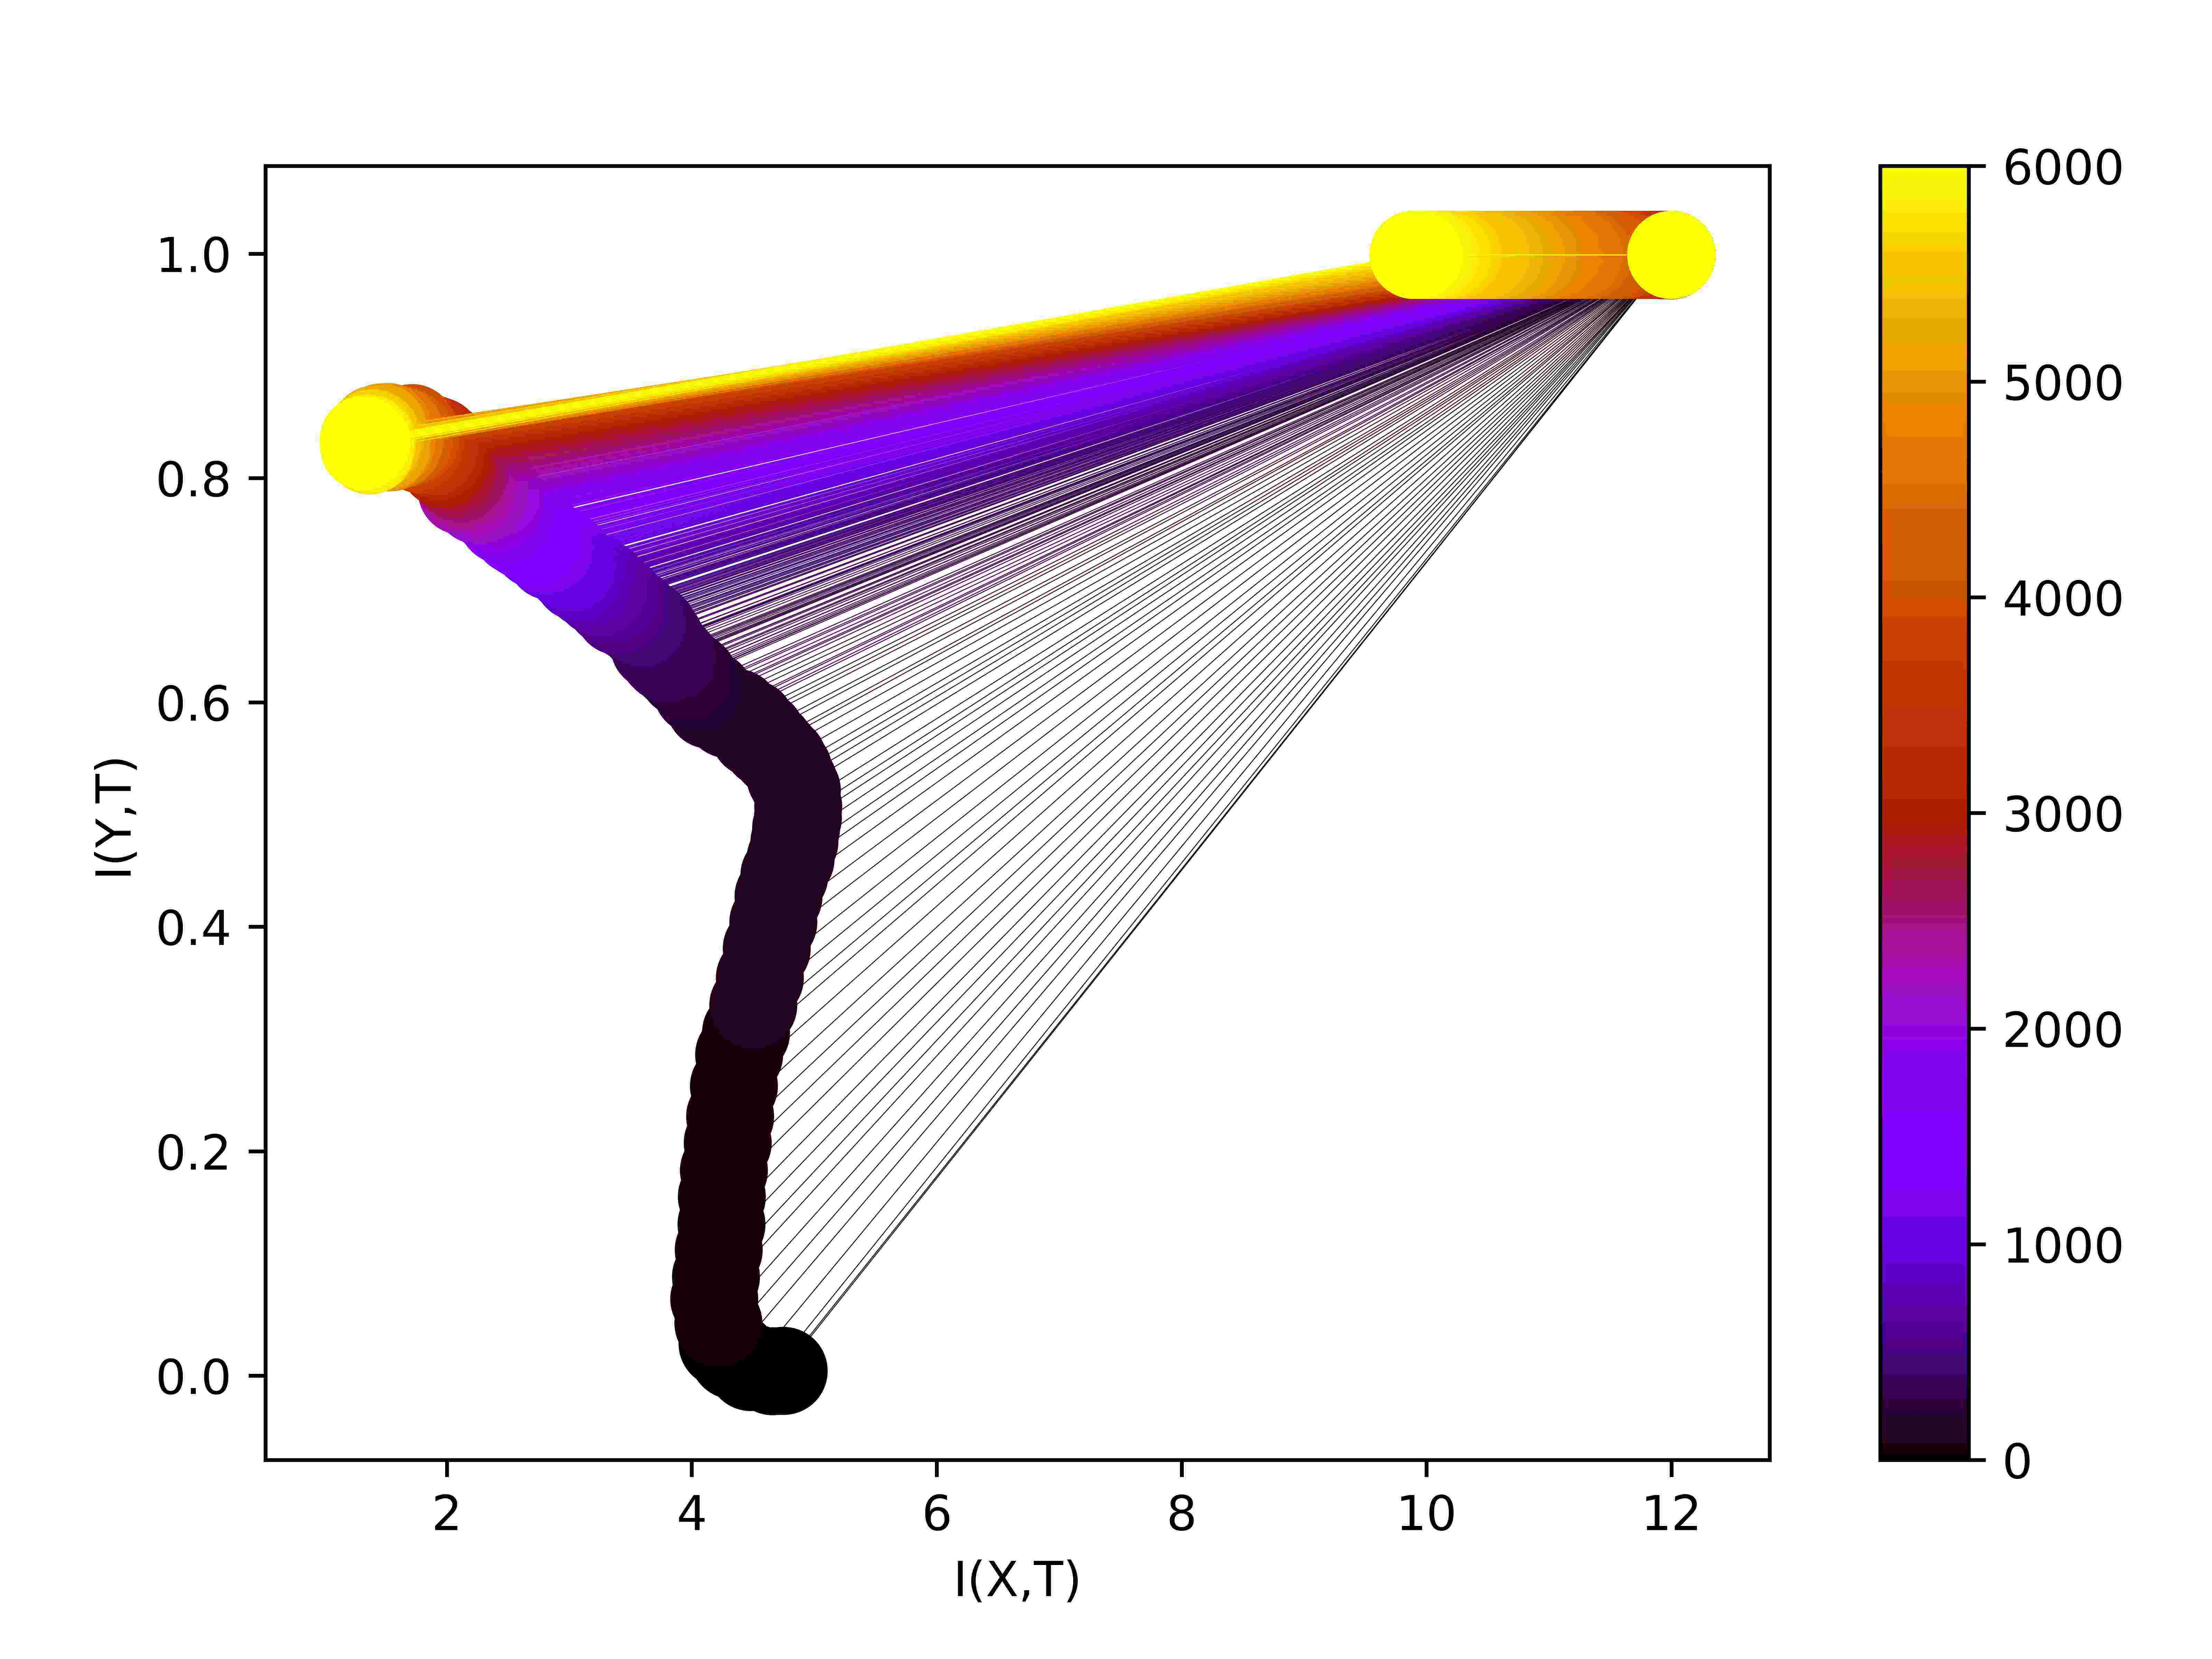
\includegraphics[width=\textwidth]{figs/eval/networkShape/Binning12,12,12.jpg}
    \caption{
      Network Shape - 12,12,12,12,2
    }
    \label{figNetworkShape3}
  \end{subfigure}
  \hfill
  \caption{
      Tweaking Network Shape for Tishby's binning MIE. 
    }
  \label{figNetworkShapes}
\end{figure}

\begin{figure}[ht]
  \begin{subfigure}[t]{0.3332\textwidth}
    \centering
    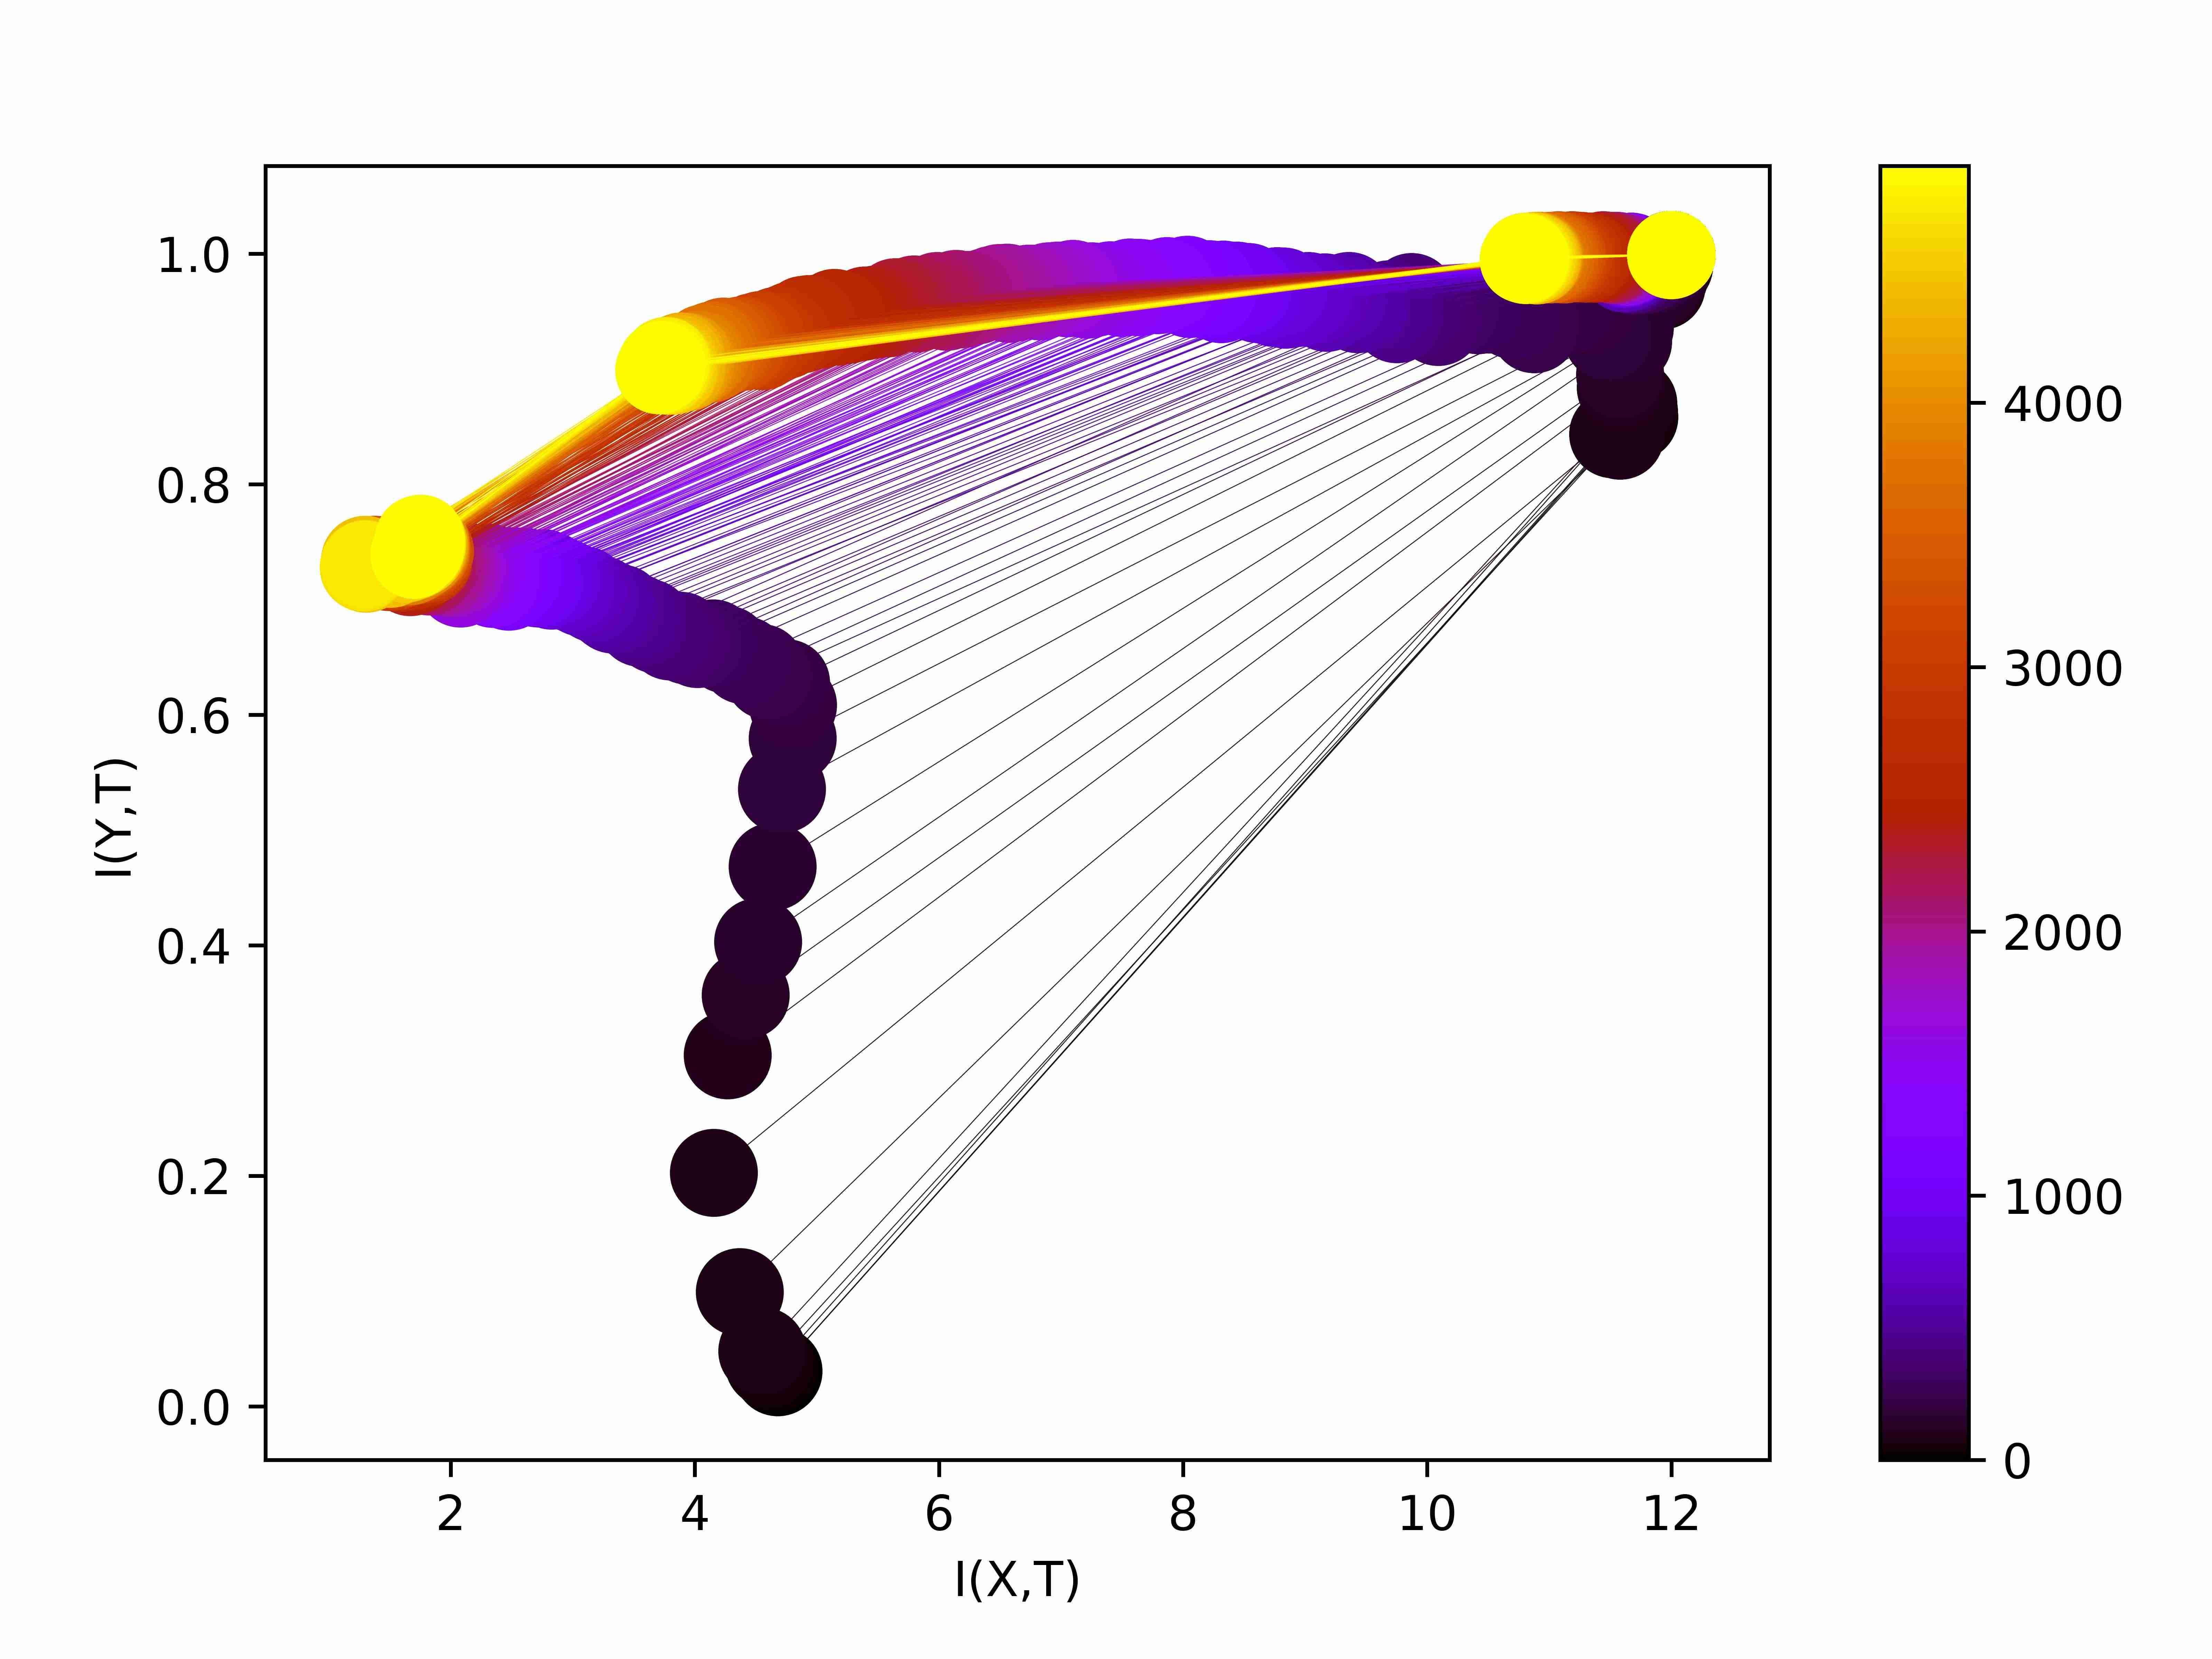
\includegraphics[width=\textwidth]{figs/eval/batchSize/Binning128.jpg}
    \caption{
      Batch size - 128
    }
    \label{figBatchSize128}
  \end{subfigure}
  \centering
  \begin{subfigure}[t]{0.3\textwidth}
    \centering
    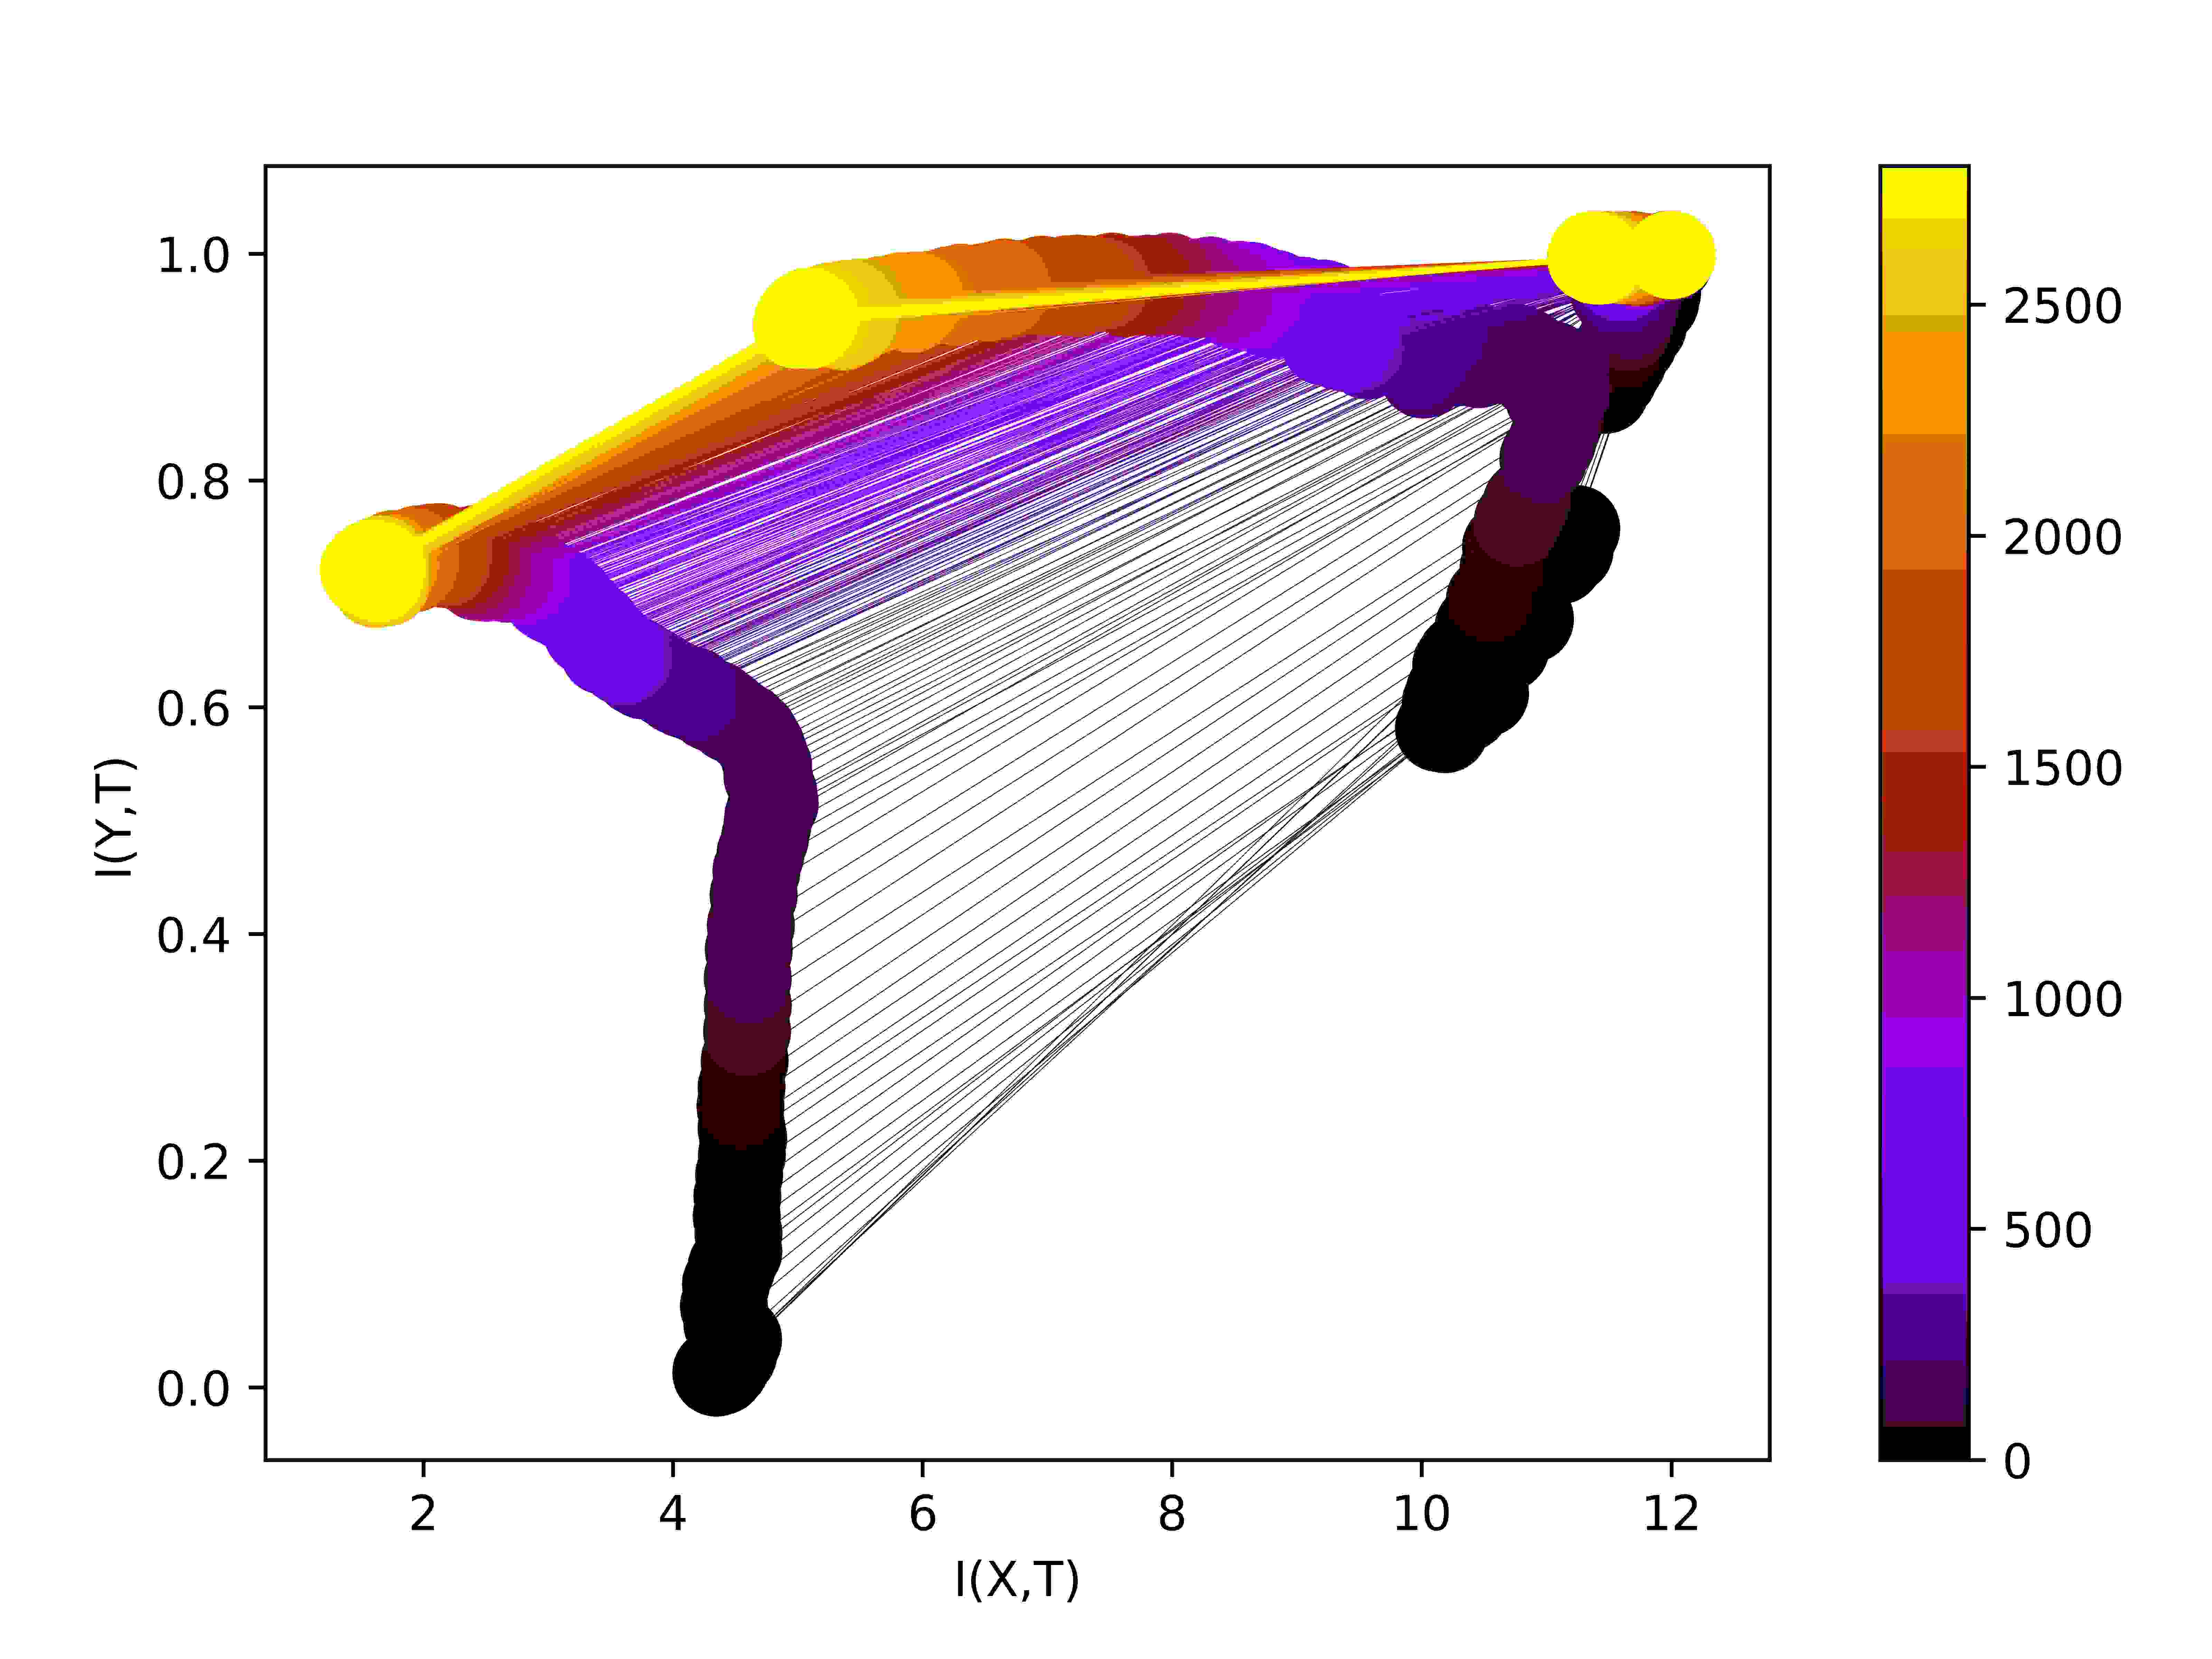
\includegraphics[width=\textwidth]{figs/eval/batchSize/Binning256.jpg}
    \caption{
      Batch size - 256
    }
    \label{figBatchSize256}
  \end{subfigure}
  \begin{subfigure}[t]{0.3332\textwidth}
    \centering
    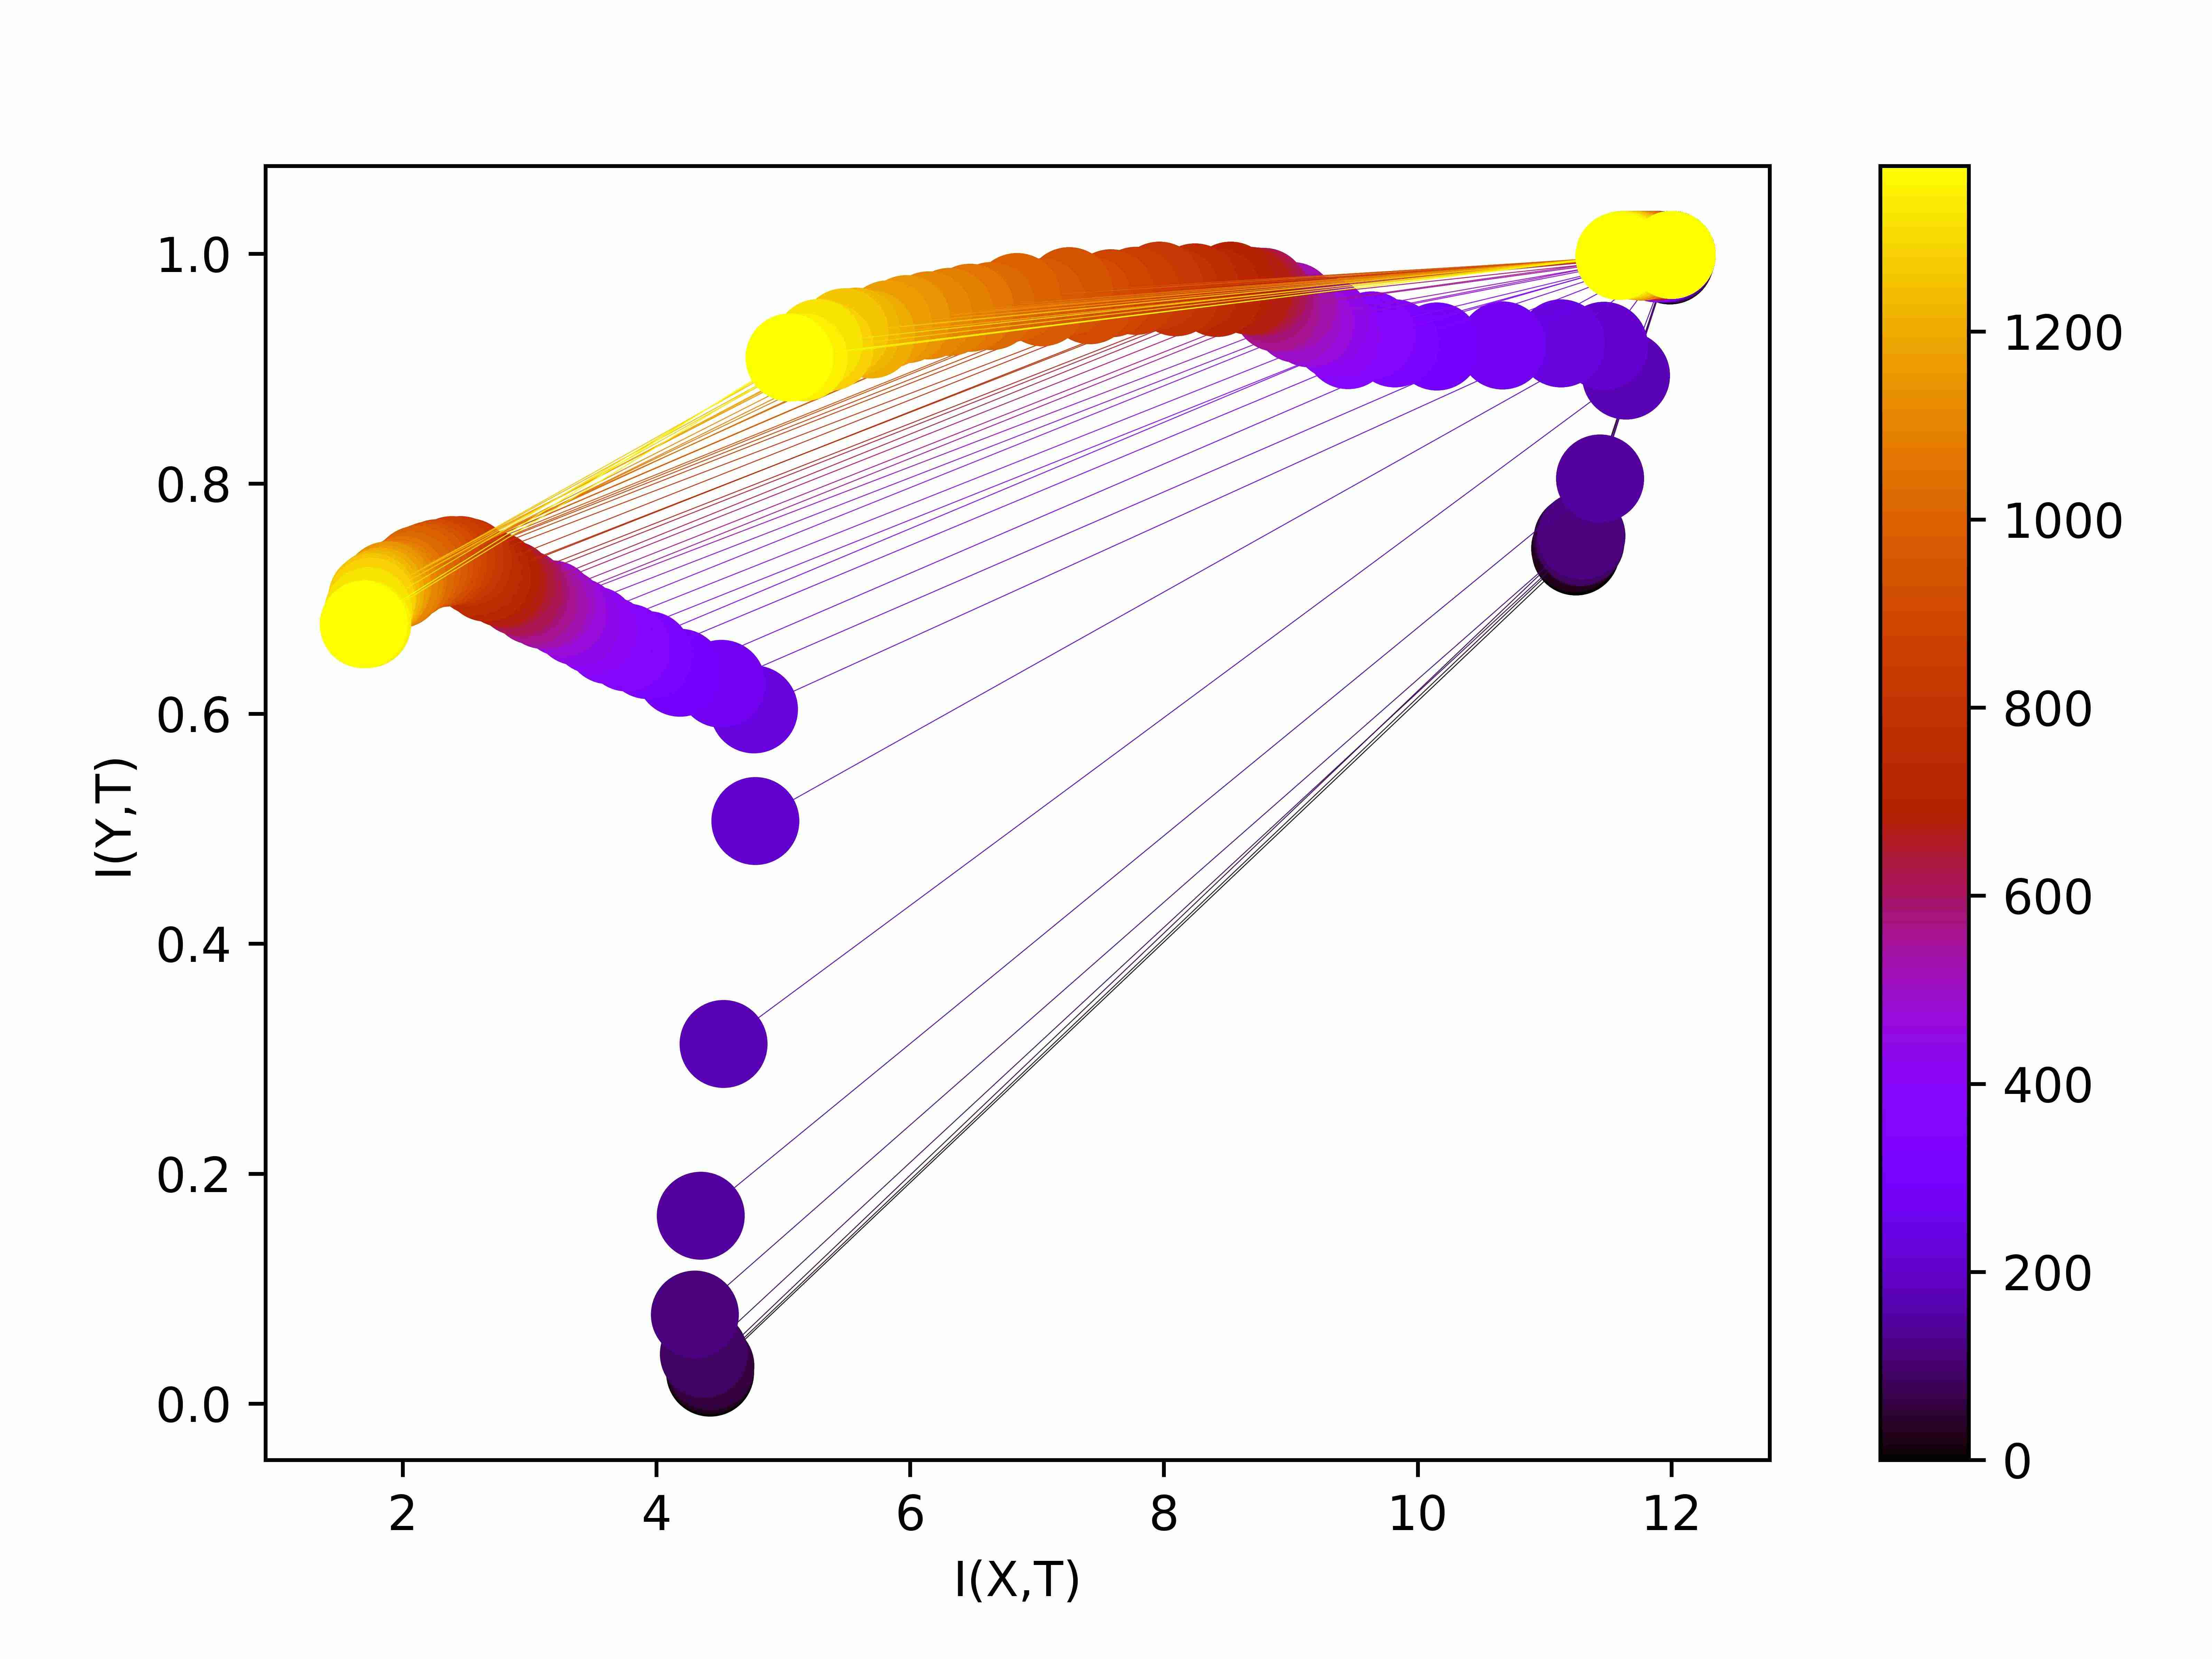
\includegraphics[width=\textwidth]{figs/eval/batchSize/Binning512.jpg}
    \caption{
      Batch size - 512, Default
    }
    \label{figBatchSize512}
  \end{subfigure}
  \caption{
      Tweaking batch size for Tishby's binning MIE. Training Size - 20\%
    }
  \label{figBatchSize}
\end{figure}

\begin{figure}[ht]
  \centering
  \begin{subfigure}[t]{0.24\textwidth}
    \centering
    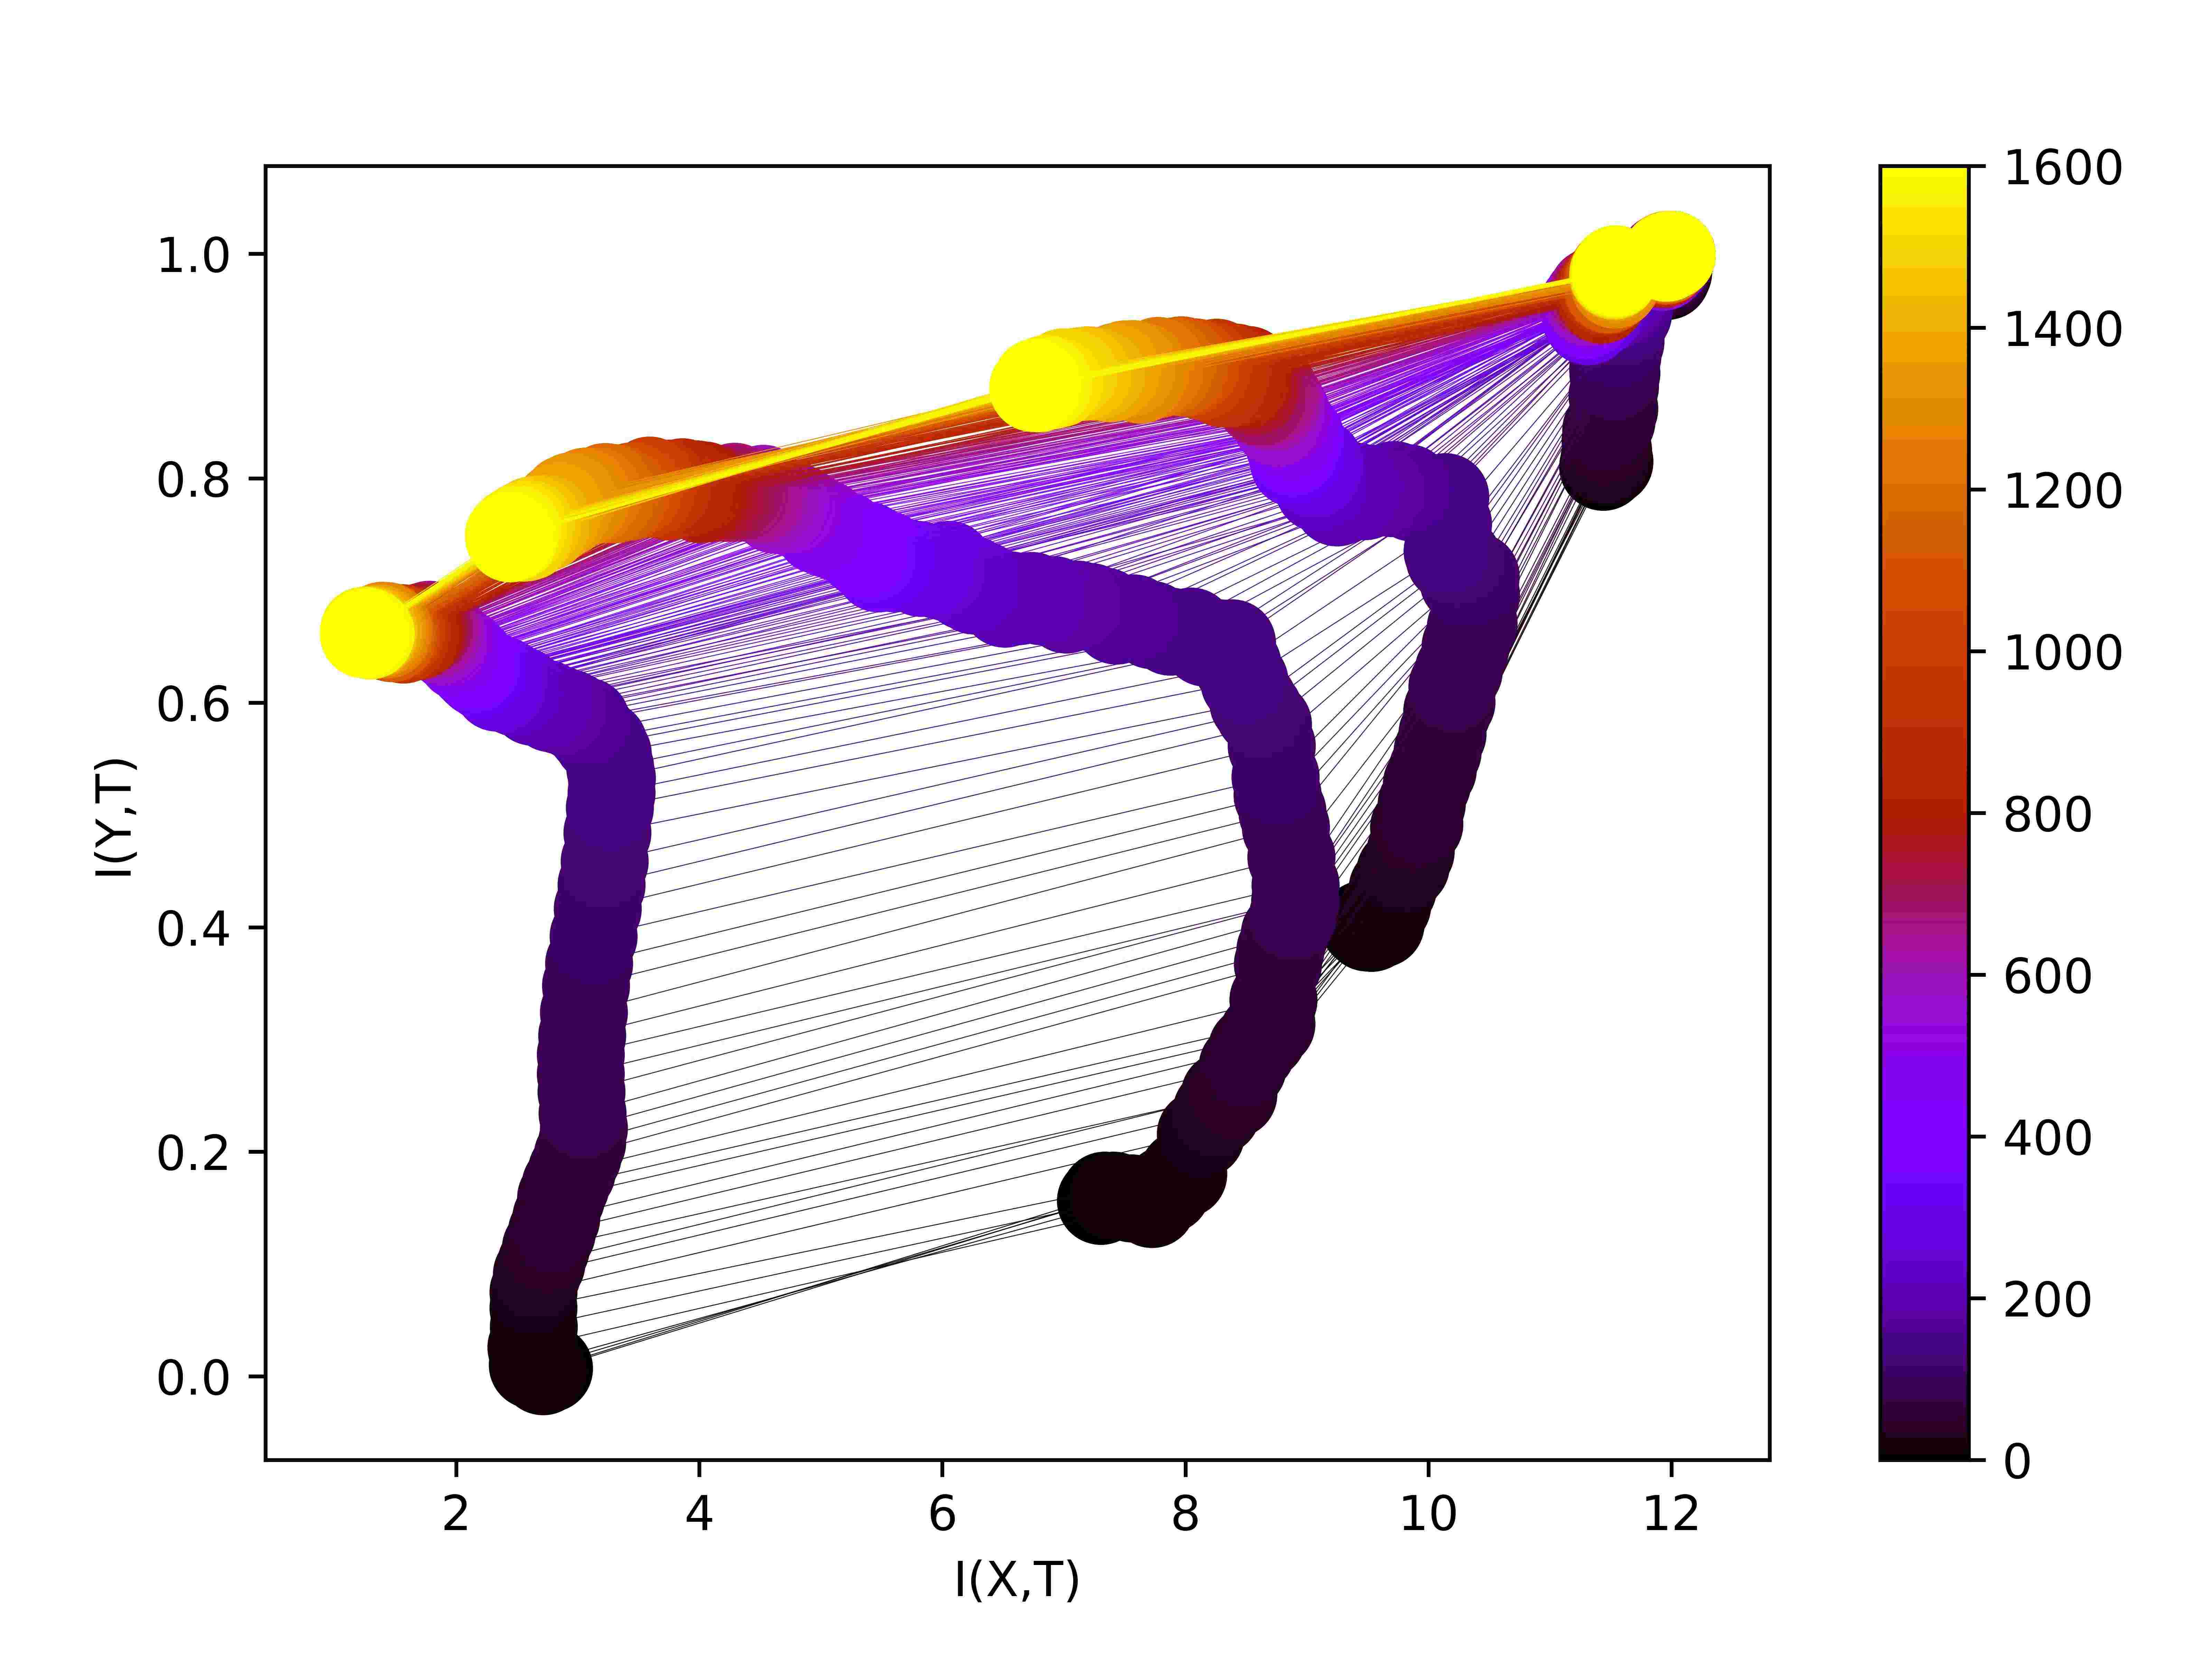
\includegraphics[width=\textwidth]{figs/eval/binCount/Binning10.jpg}
    \caption{
      Bin Count - 10
    }
    \label{figBinCount10}
  \end{subfigure}
  \hfill
  \begin{subfigure}[t]{0.24\textwidth}
    \centering
    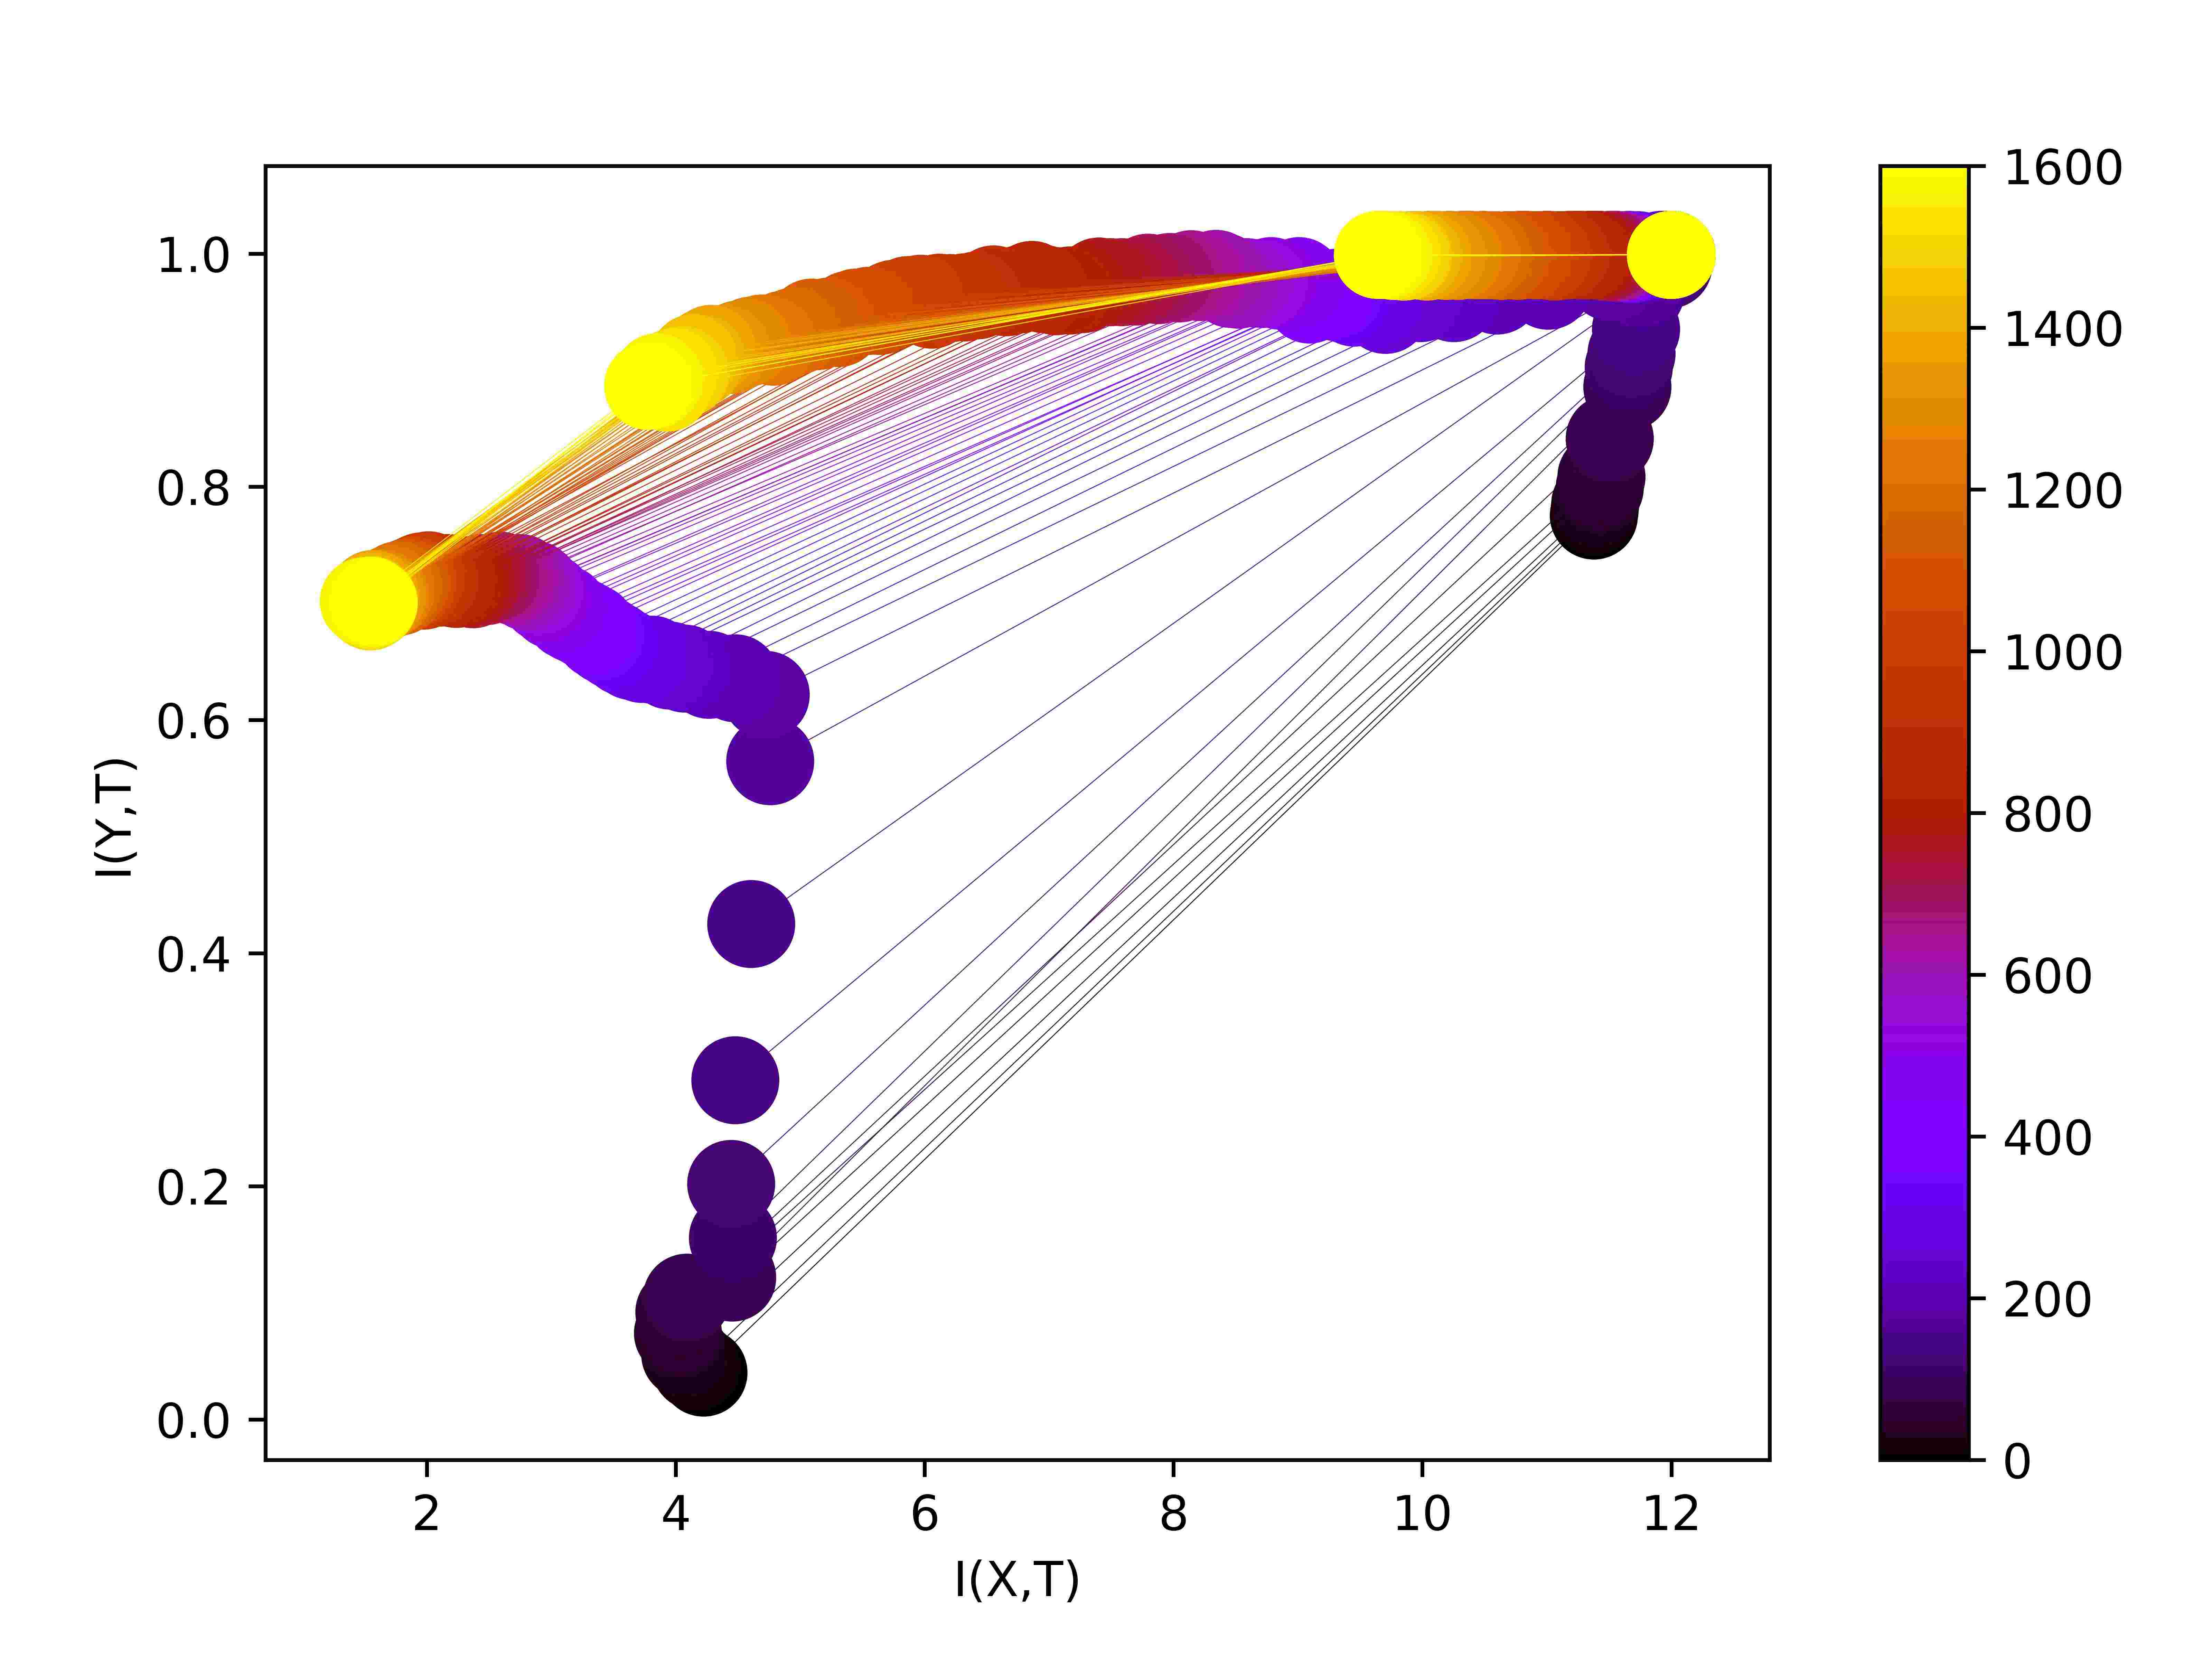
\includegraphics[width=\textwidth]{figs/eval/binCount/Binning30.jpg}
    \caption{
      Bin Count - 30, Default
    }
    \label{figBinCount30}
  \end{subfigure}
  \hfill
  \begin{subfigure}[t]{0.24\textwidth}
    \centering
    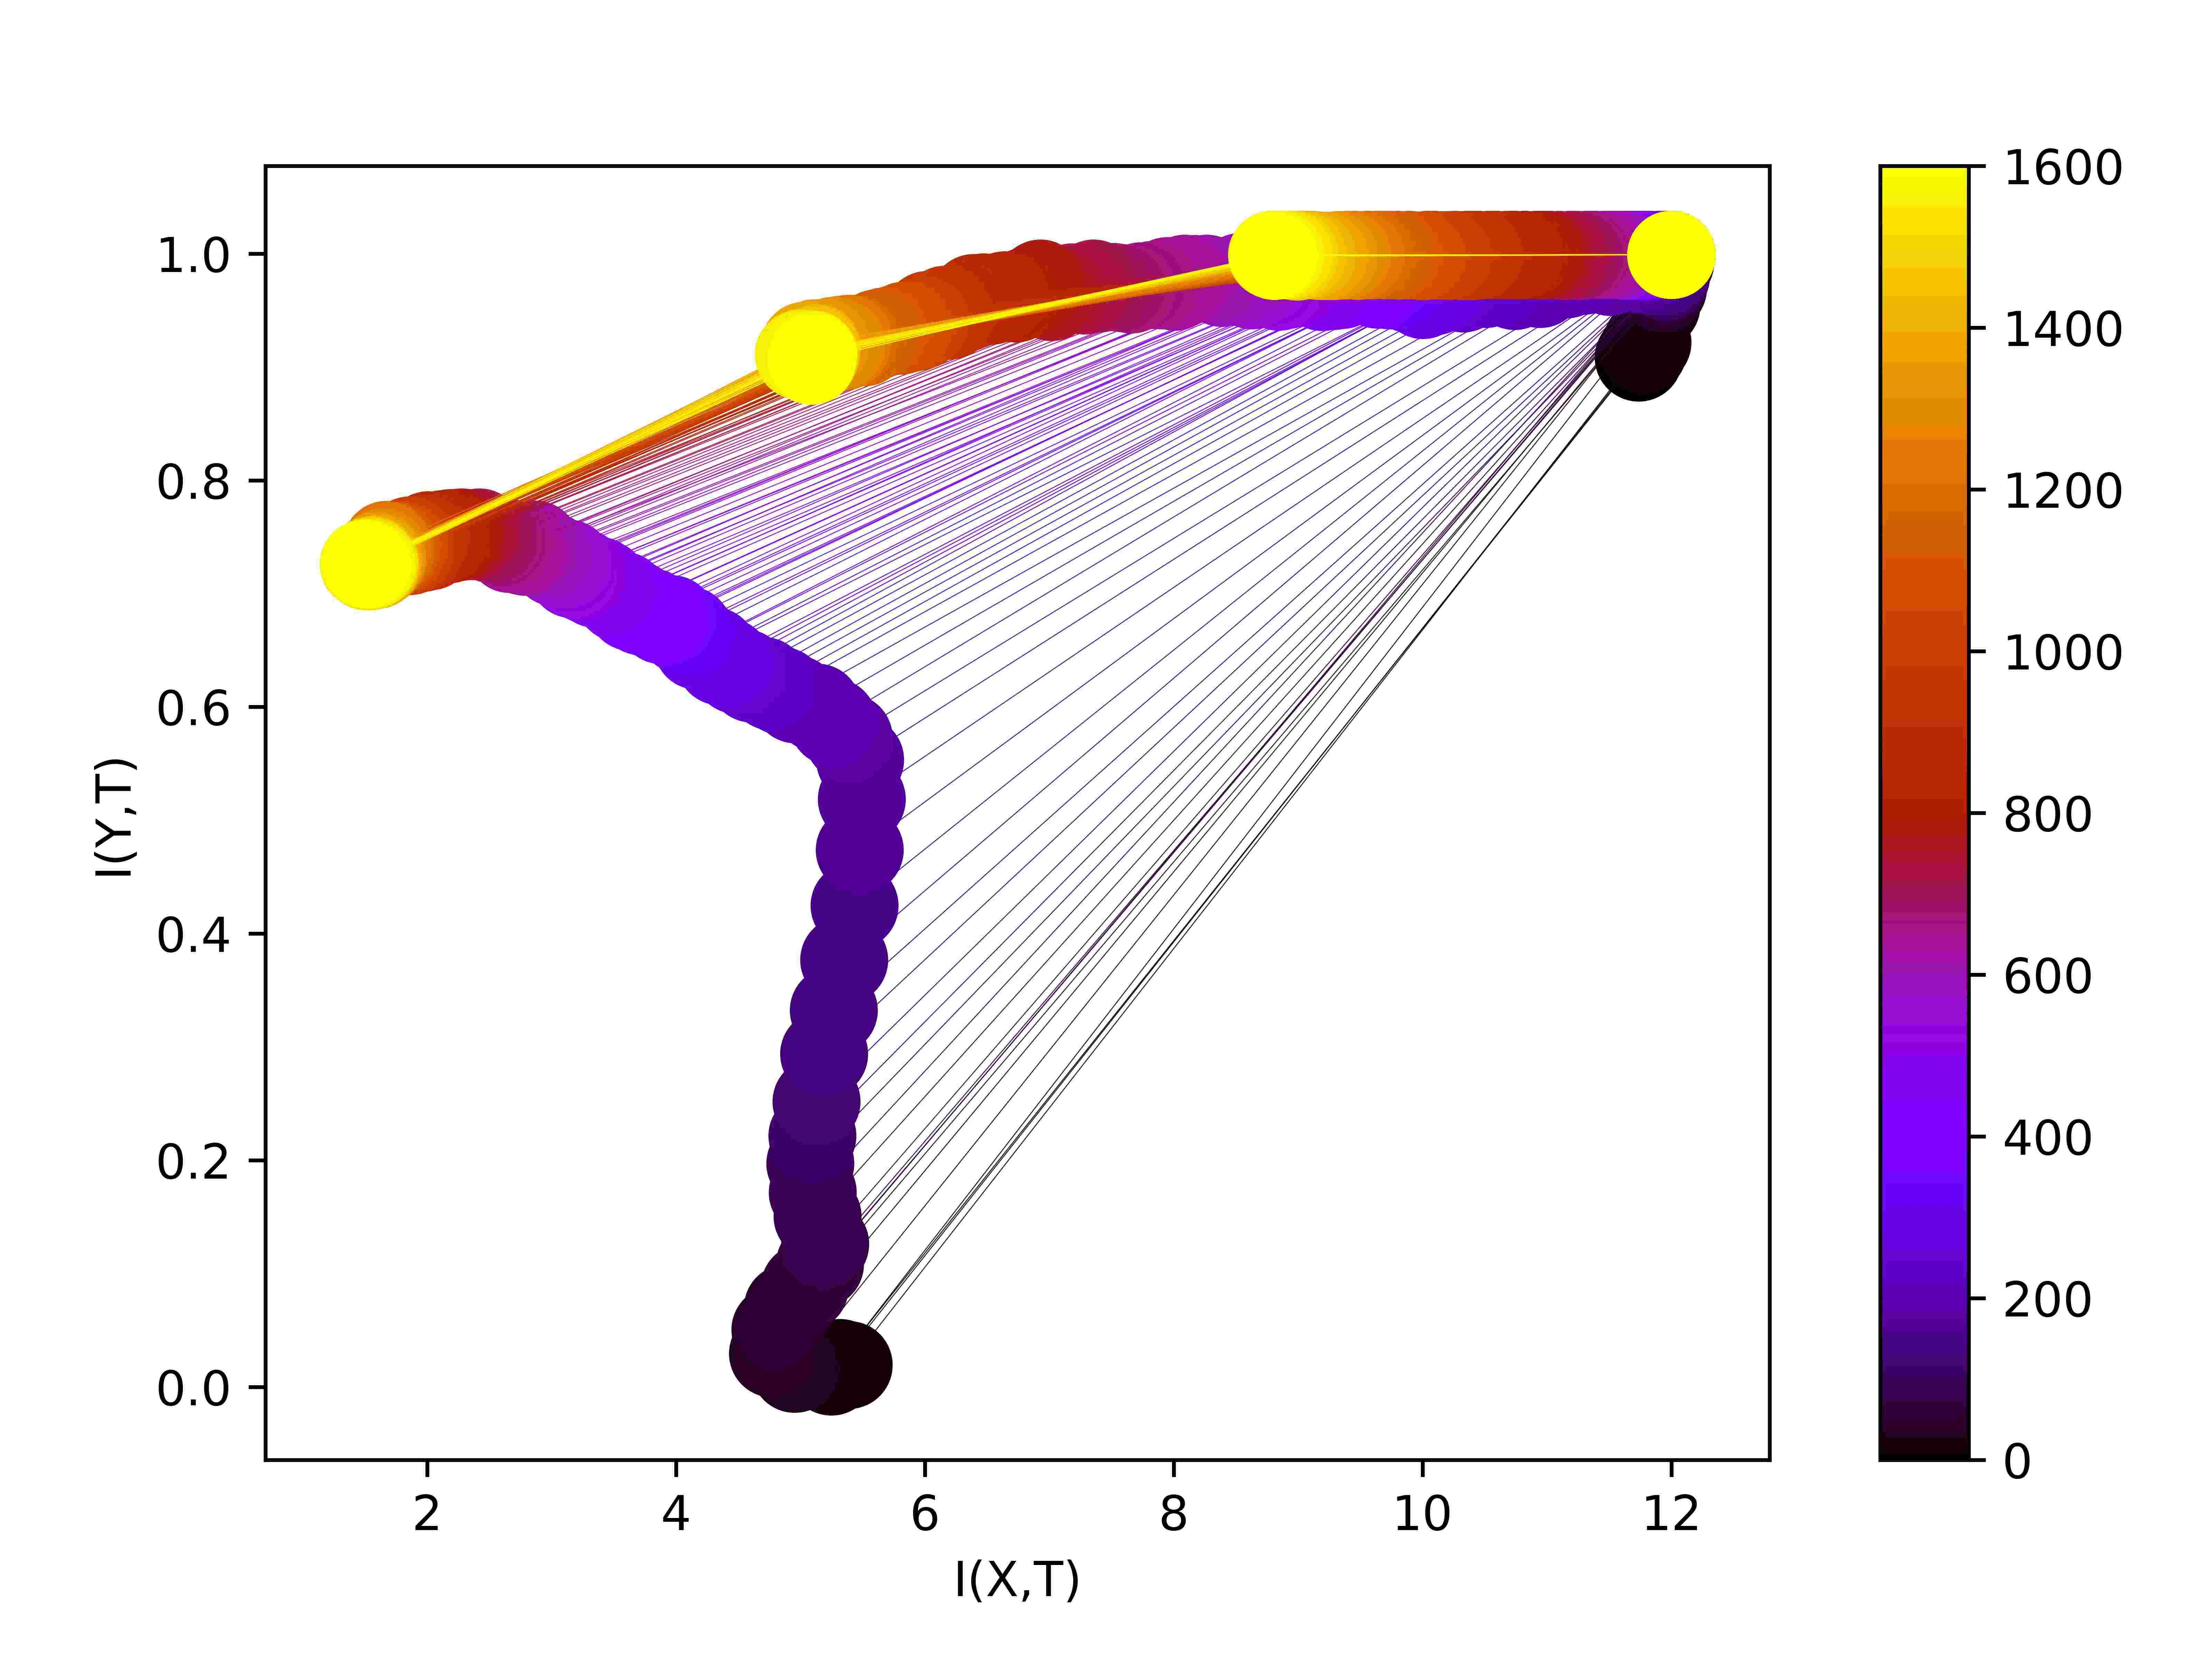
\includegraphics[width=\textwidth]{figs/eval/binCount/Binning50.jpg}
    \caption{
      Bin Count - 50
    }
    \label{figBinCount50}
  \end{subfigure}
  \hfill
  \begin{subfigure}[t]{0.24\textwidth}
    \centering
    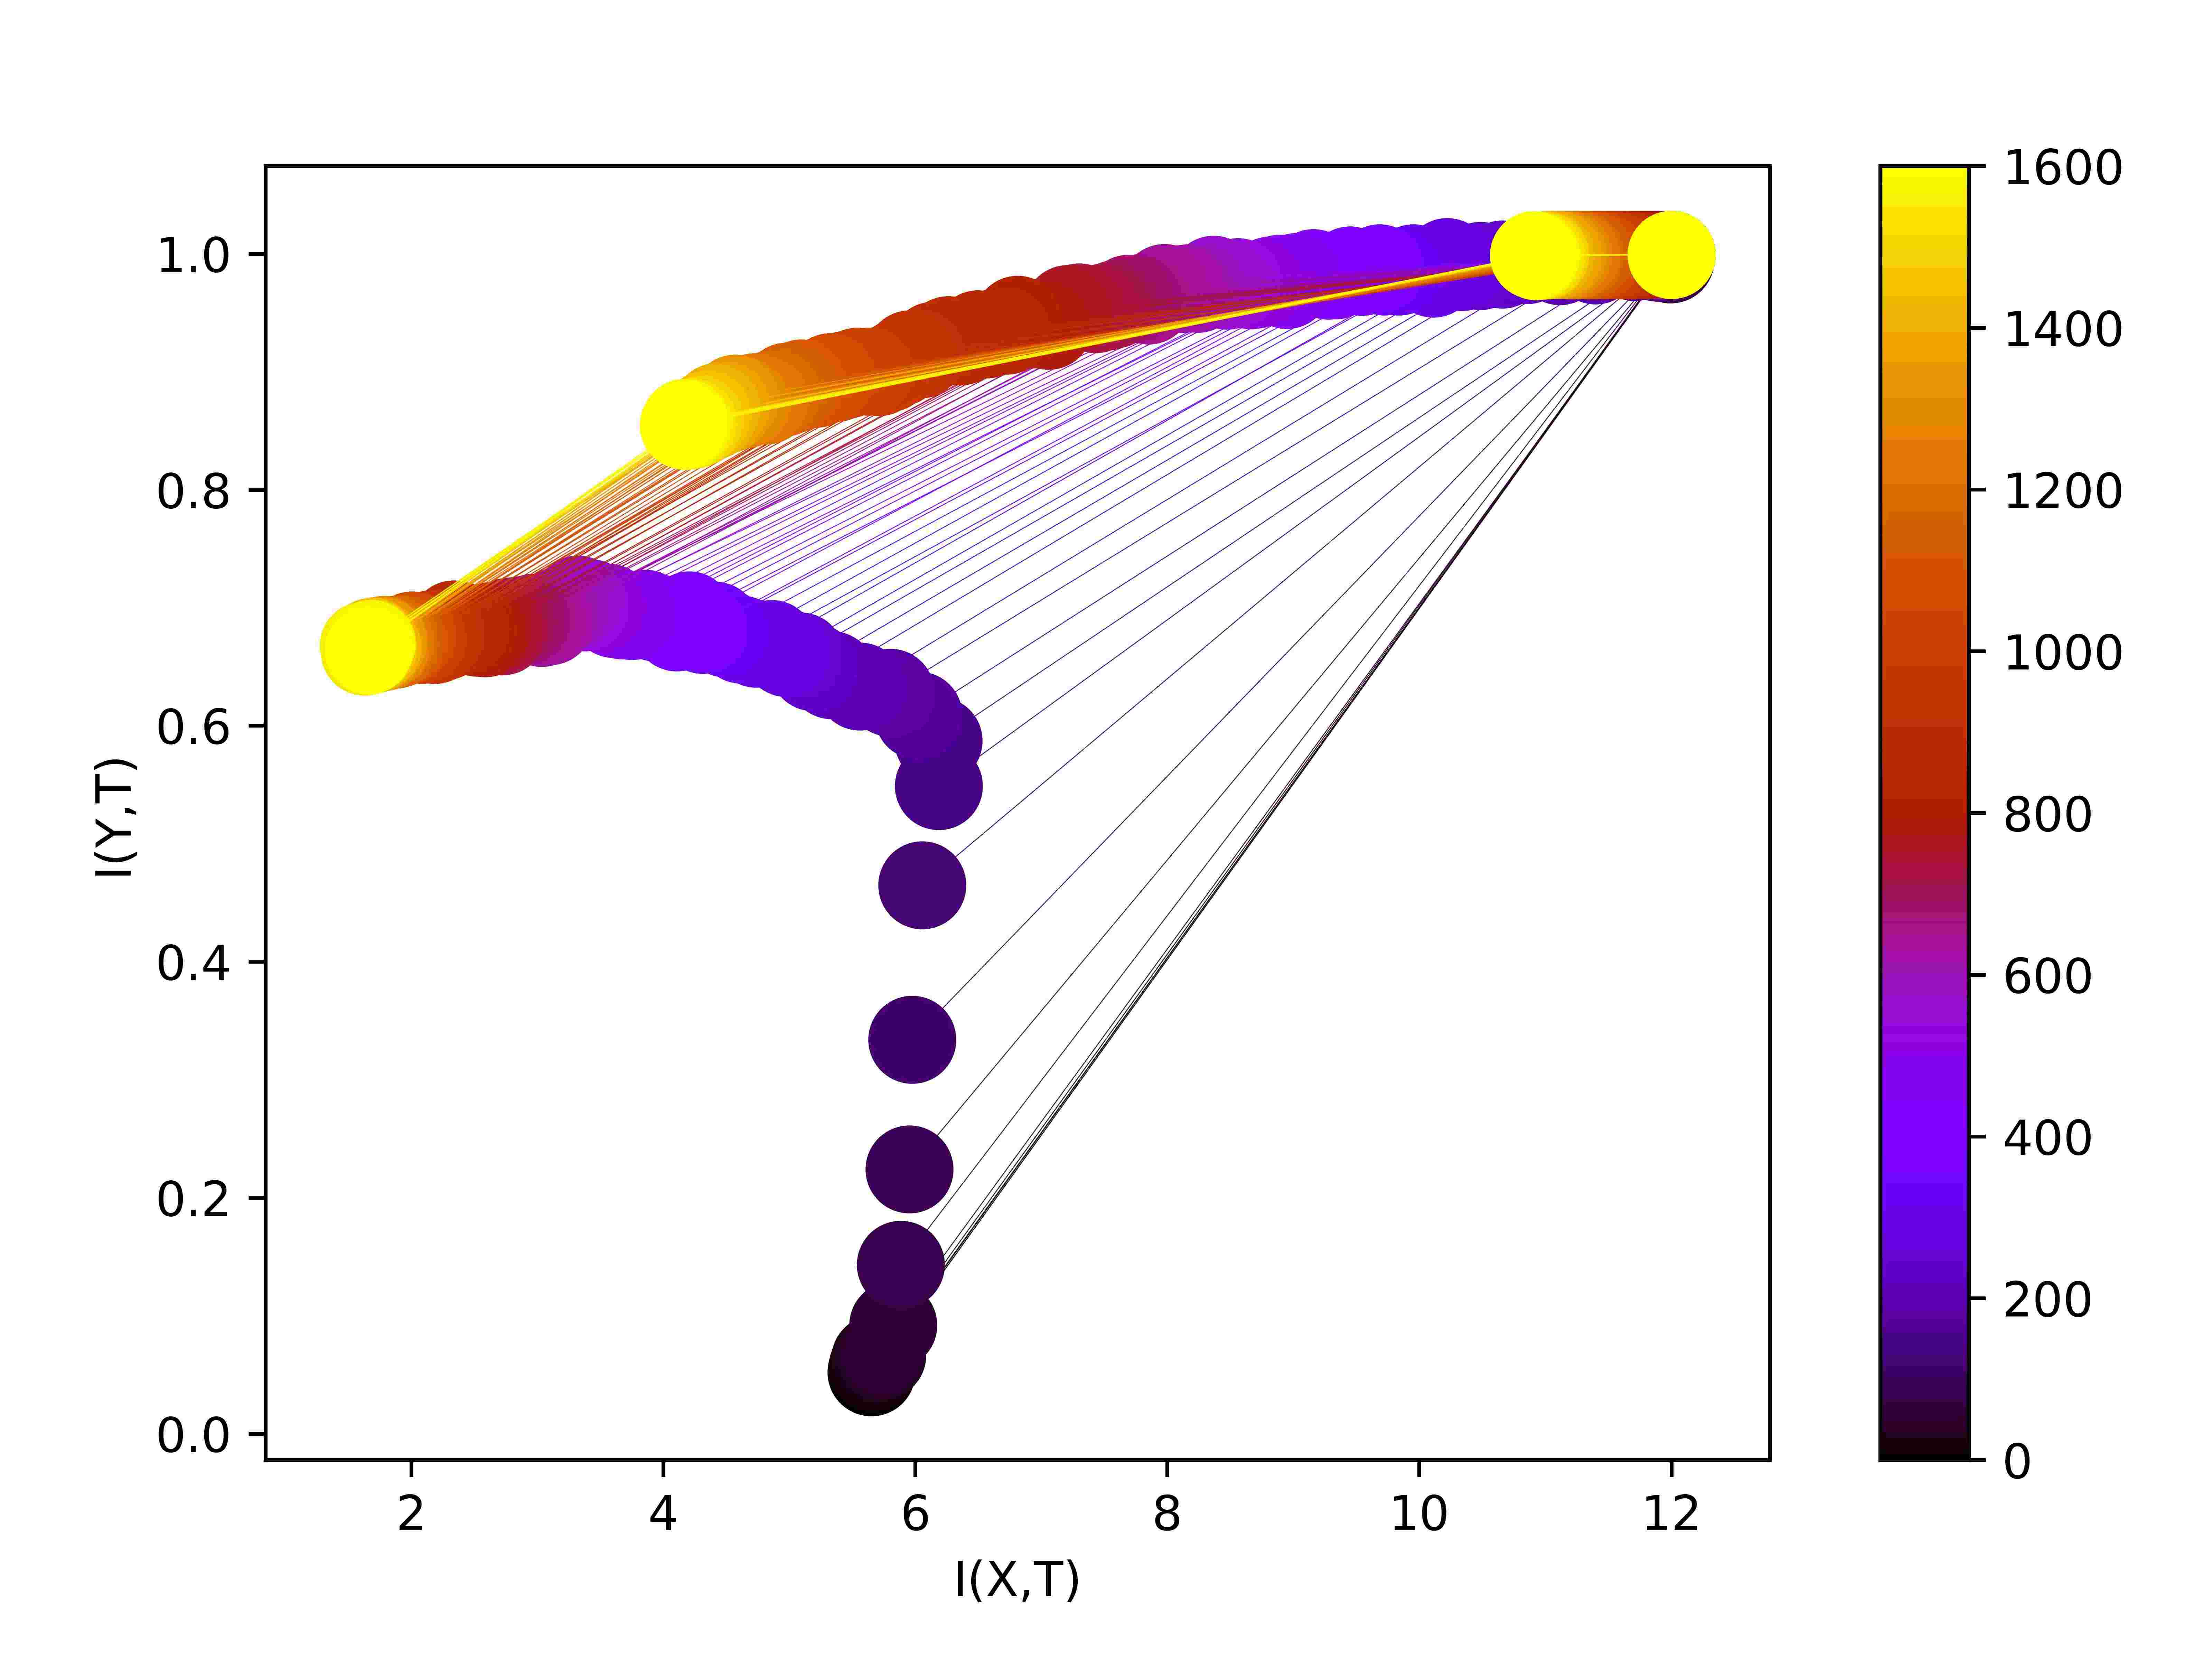
\includegraphics[width=\textwidth]{figs/eval/binCount/Binning80.jpg}
    \caption{
      Bin Count - 80
    }
    \label{figBinCount80}
  \end{subfigure}
  \hfill
  \caption{
      Tweaking bin count for Tishby's binning MIE. Training Size - 20\%. 
    }
  \label{figBinCount}
\end{figure}


\subparagraph{A note on activation functions} In every figure here the last
layer has the activation function $softmax$, so if we change the activation
function we should ignore the last layer as it might be misleading.

\subsection{Saxe's experiment and the activation function} \label{subEvalSaxe}

In his Paper Saxe claimed that Tishby's results are an epiphenomena of the
activation function $tanh$ and compression phase does not happen if we use the
ReLu activation function. Let us look at his experiments:
\begin{itemize}
  \item{
      The First one used the KDE as the MI estimator, and set the activation
      function to ReLu. All other values as default.
    }
  \item{
      And the second one used the KDE as the MI estimator, ReLu as the
      activation function, and MNIST as the dataset. All other values as default
    }
\end{itemize}
Notice that both of the experiments, changes MIE and the activation changes MIE
and the activation function at the same time. However, If we tweak only the
activation function while leaving MIE to be Binning we get the results present
in \autoref{figReluTanh}
\begin{itemize}
  \item{
      Tanh - we see the usual results.
    }
  \item{
      ReLu - we see a completely different Information Plane. We can clearly see
      see signs of a Compression phase. However, it is not as pronounced
      as for the Tanh activation. This result goes against the claims proposed
      by Saxe -- that ReLu function does not produce a compression phase.
      Furthermore this results does not support Tishby's claims as the
      Information plane is missing the Fitting phase.
    }
\end{itemize}
According to Saxe a NN with activation ReLu does not have a compression phase --
a claim that \autoref{figReluTanhRelu} goes against. The discrepancy arises when
we use different MI Estimators: in our case KDE and Binning. I suspect that one
or both of these estimators are misleading. I did not provide a plot for the KDE
MIE as there are slight discrepancies between my results and results of Saxe --
even though I have used used their implementation of KDE. As I was not able to
detect the source of the discrepancies I decided against including it here, see
\autoref{appendixKDE}.


\begin{figure}[ht]
  \centering
  \begin{subfigure}[t]{0.49\textwidth}
    \centering
    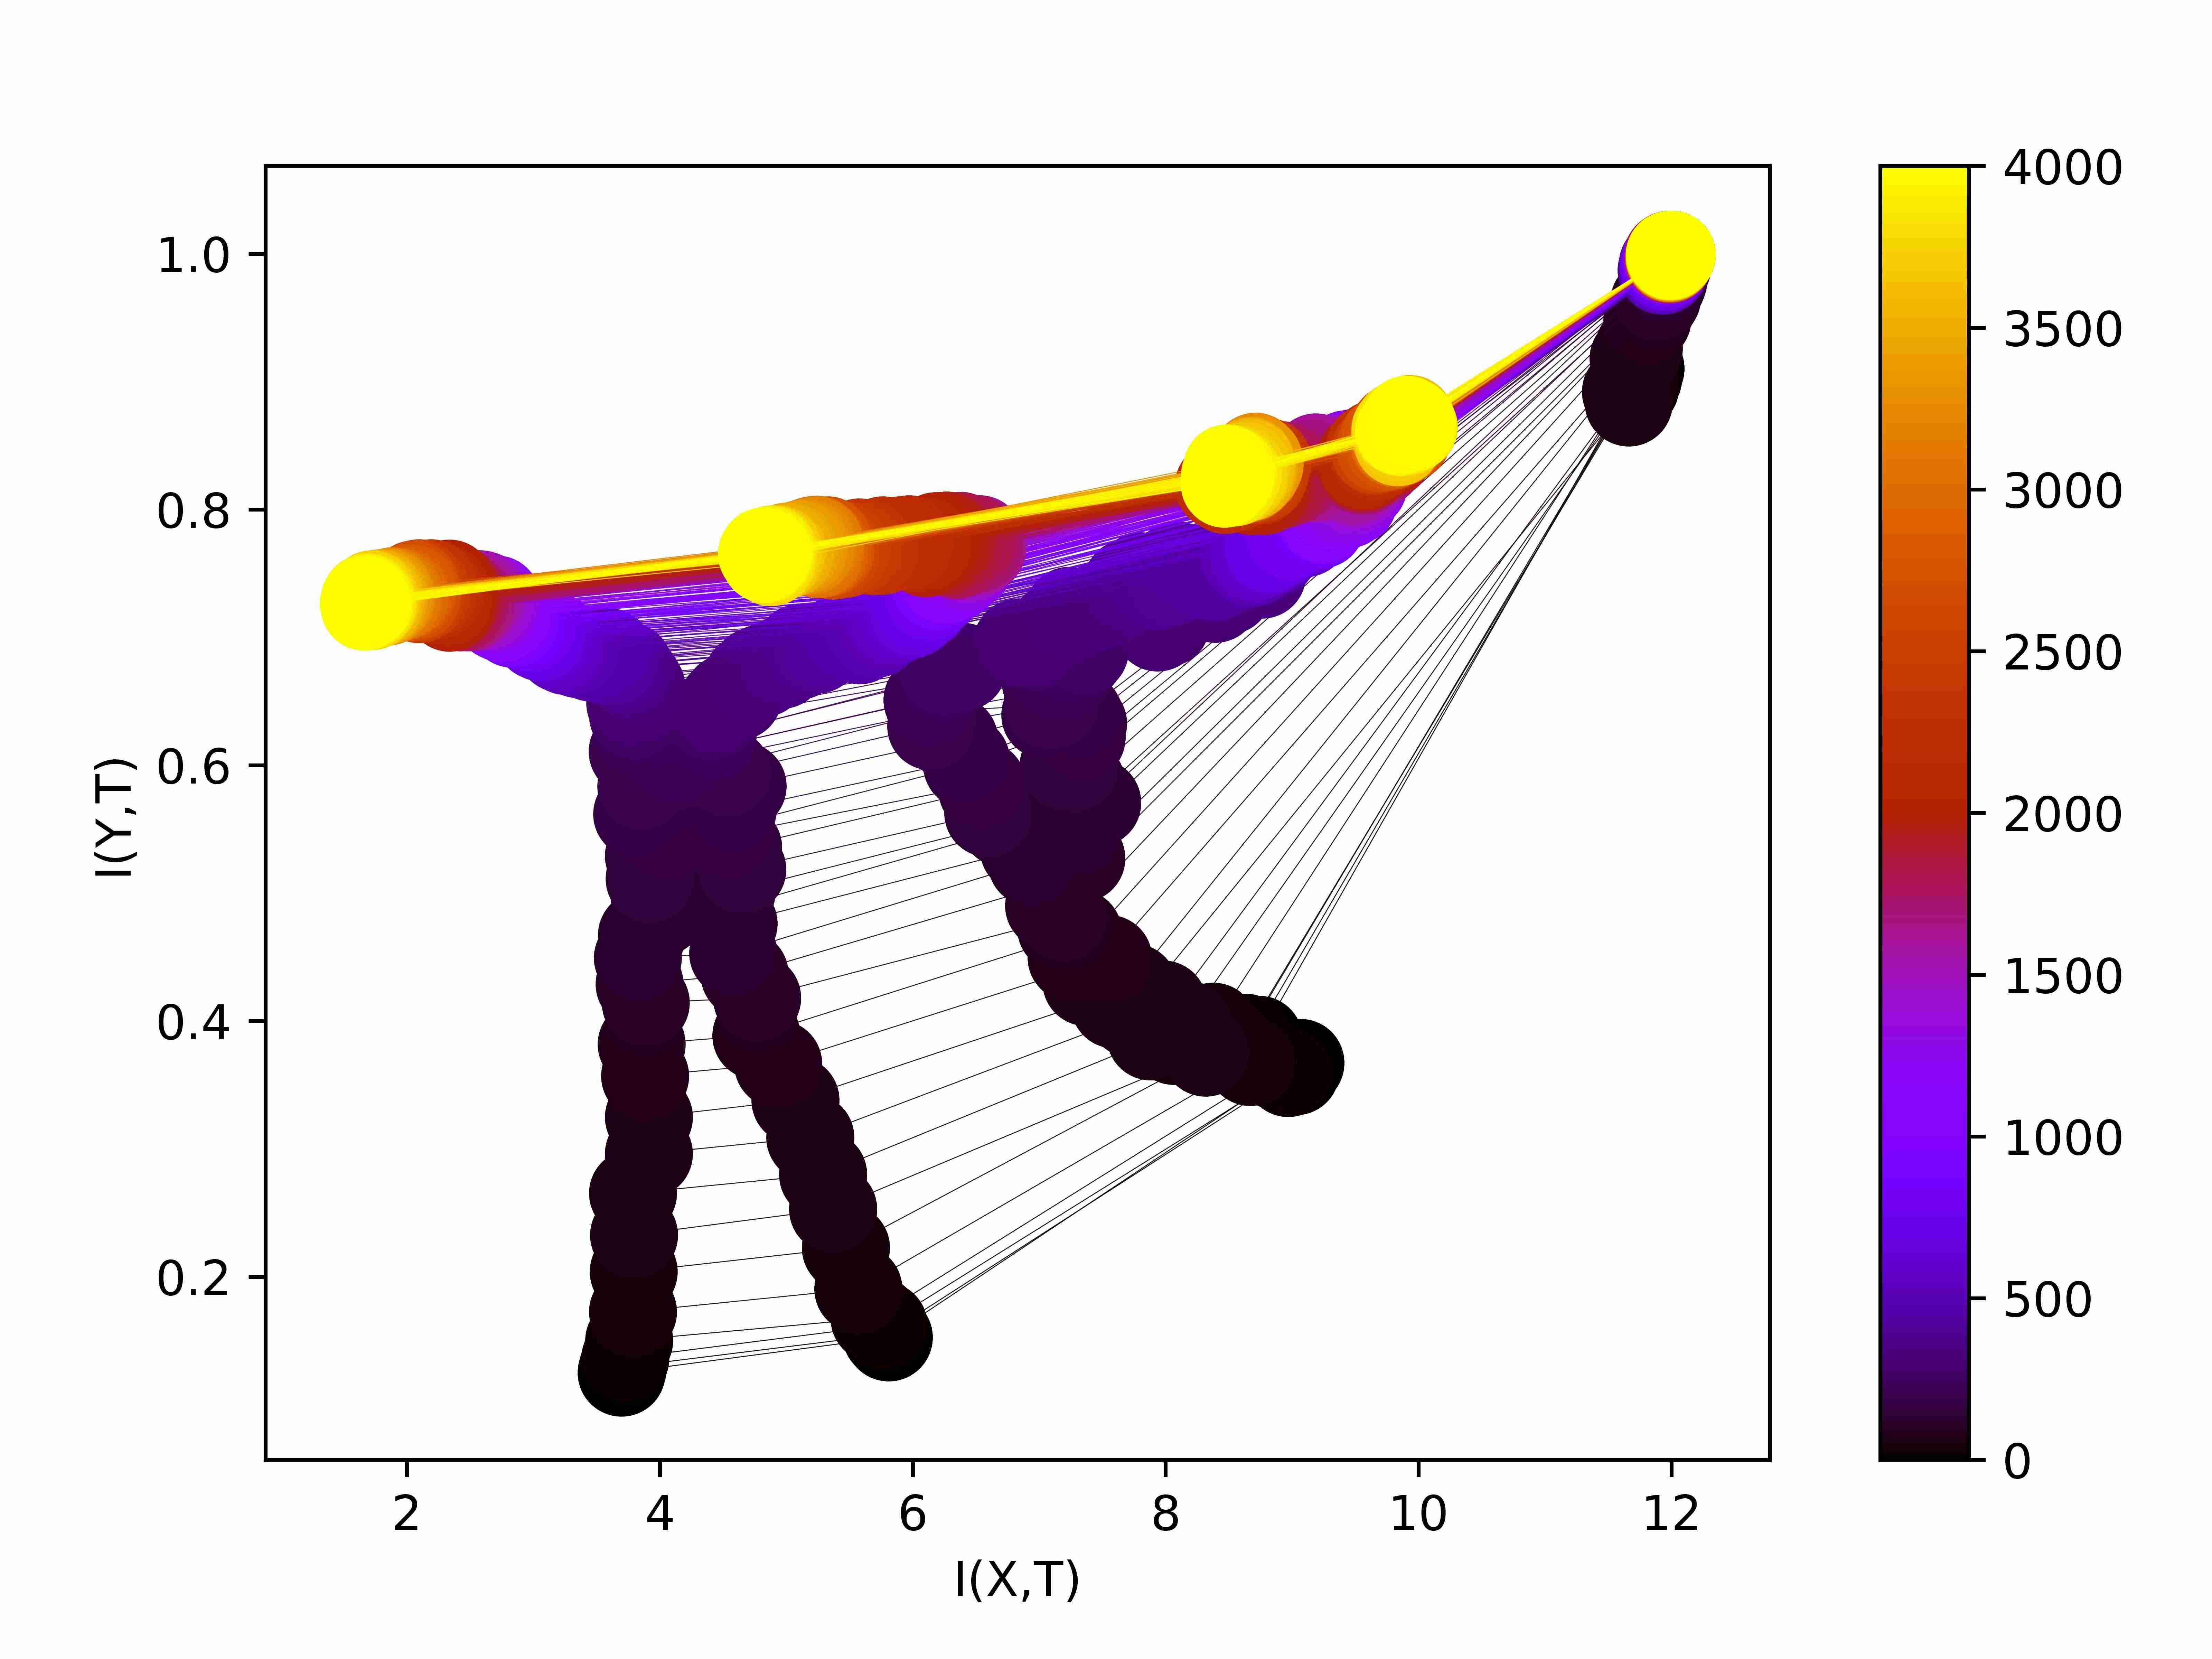
\includegraphics[width=0.7\textwidth]{figs/eval/activationFunction/BinningRelu.jpg}
    \caption{
      MIE - Binning, activation function - ReLu
    }
    \label{figReluTanhRelu}
  \end{subfigure}
  \begin{subfigure}[t]{0.49\textwidth}
    \centering
    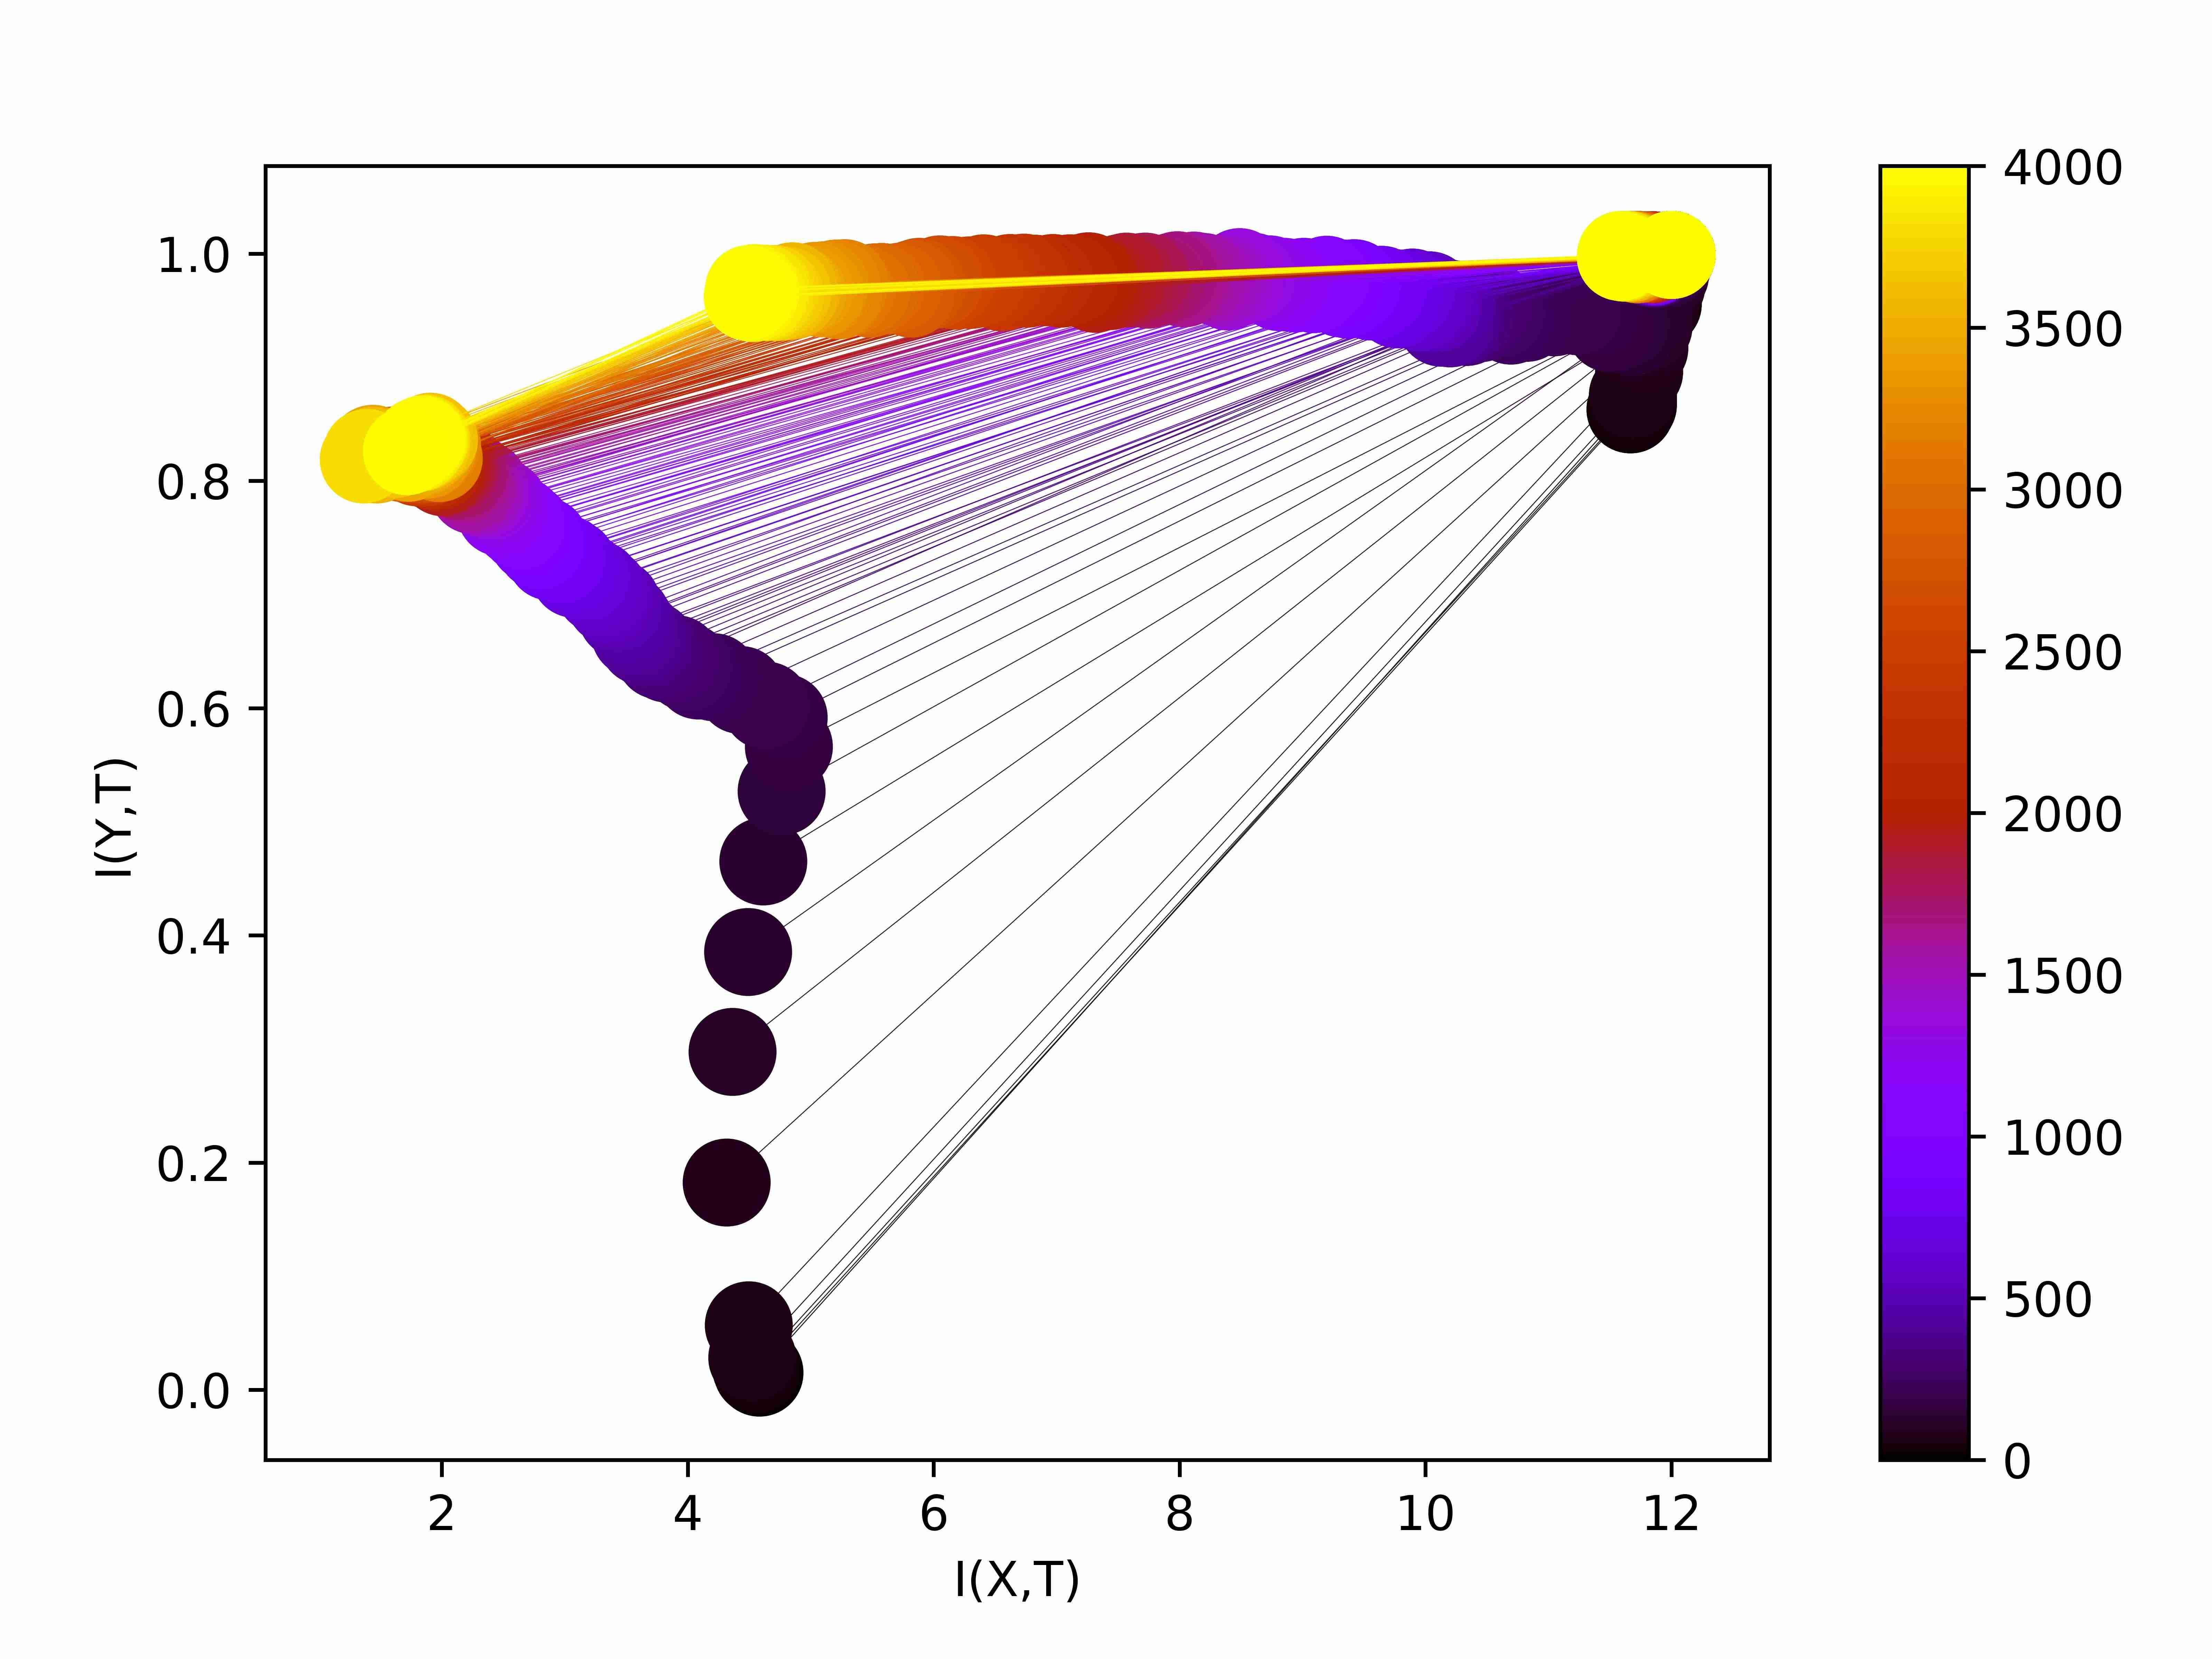
\includegraphics[width=0.7\textwidth]{figs/eval/activationFunction/BinningTanh.jpg}
    \caption{
      MIE - Binning, activation function - $\tanh$
    }
    \label{figReluTanhTanh}
  \end{subfigure}
  \caption{
      Tweaking the activation function, ignore the last layer as it's
      activation function cannot be changed.
    }
  \label{figReluTanh}
\end{figure}

\section{Batching} \label{subEvalBatching}

Motivation for deriving the batching MIE was the discovery of disagreements
between the two methods: Binning and KDE. The disagreement implied that methods
currently used do not provide enough precision in order to answer questions
proposed. Such as is the compression inherent in to the NN.  Deriving a novel
method of mutual information estimation was beyond this project. Instead a
better way was to use properties of the NN to explore ways how we can improve
performance of an exists in method to estimate MI. 

The tool batches multiple epochs together therefore, it is not fit to answer
questions that ask about how information plane changes from epoch to epoch.
This includes questions about the Compression phase and the Fitting phase.  It
is a tool specifically made to get a better estimate for one instance. As such it
is difficult to evaluate, as to do so we would need to know true information
values inside the NN.

\section{Ending remarks}

In this project we have explored the assumptions that need to be made in order
for NN to compress information.  We investigated Binning and KDE: tools that
estimate the level of compression in a different ways.  We showed that tat
Binning is robust to some parameter changes.  However, robust does not imply
correct.  We discovered that the reason why Tishby and Saxe disagree, might be
because their tools give different answers in specific situations.  I think
there needs to be more work done to improve the tools being used.  It would be
interesting to understand why Binning and KDE produce differing results when the
activation function is ReLu. This work needs to be done, before we can answer
fundamental question about Neural Networks 

\end{document}
